%%==================================================
%% chapter02.tex for SJTU Master Thesis
%% based on CASthesis
%% modified by wei.jianwen@gmail.com
%% version: 0.3a
%% Encoding: UTF-8
%% last update: Dec 5th, 2010
%%==================================================

% \bibliographystyle{sjtu2} %[此处用于每章都生产参考文献]

\chapter{信道状态采样与估计}
\label{chap:phy}

安全始终是高速铁路发展过程中的首要目标,而GSM-R网络则是保证高铁系统安全性的重要环节,因此有必要对GSM-R网络进行在线实时测试,在确保GSM-R网络正常通信的基础之上,保证整个高铁系统的稳定运行。但是由于高铁系统具有较为特殊的无线传播环境,传统的信号强度测试算法无法直接应用于GSM-R网络测试中,例如高铁线路周围地形复杂多变以及列车处于高速运行状态,这就要求GSM-R网络信号强度测试算法必须具有实时高效的特点,以适应高速铁路的特殊要求。

\begin{figure}[!htp]
\centering
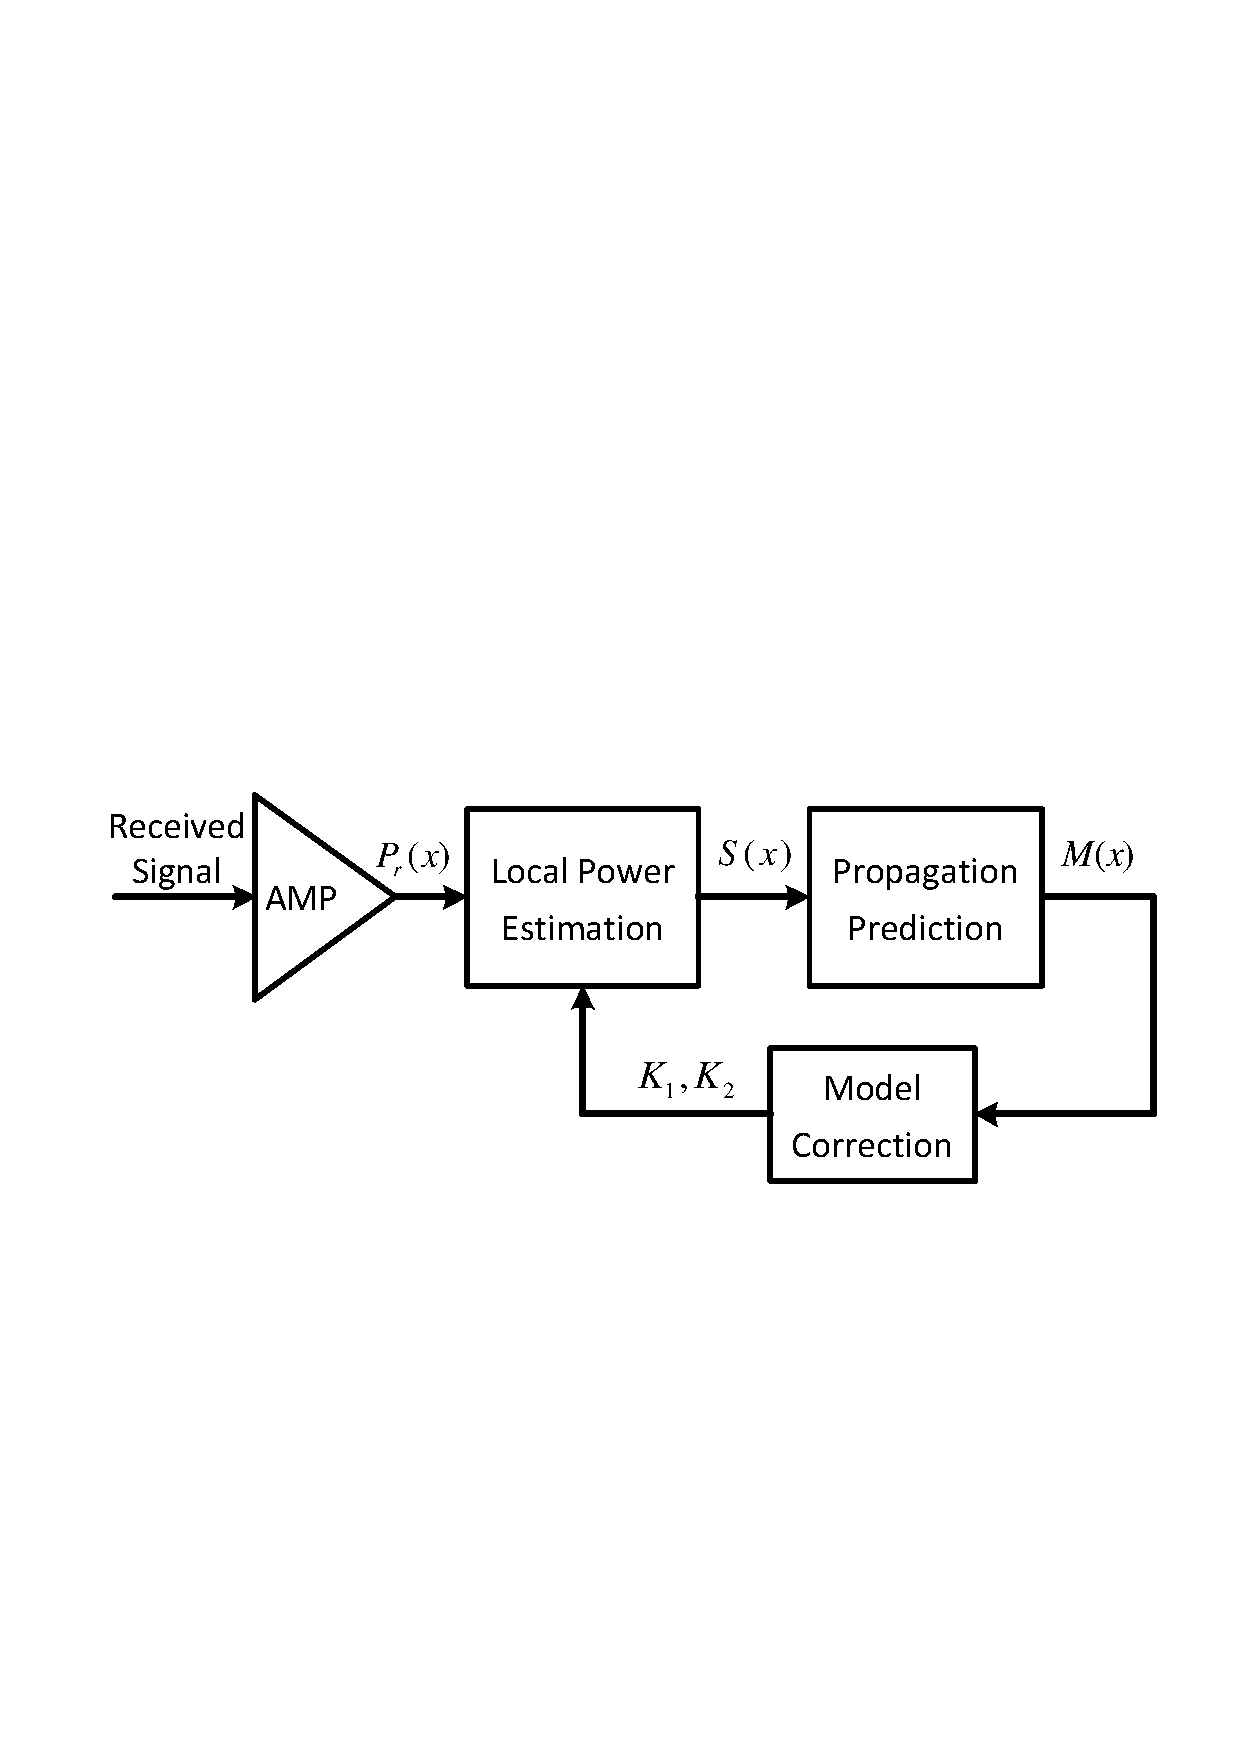
\includegraphics[width=4in]{chap2/measurement.pdf}
\bicaption[fig:measurement]{接收信号强度测试过程}{接收信号强度测试过程}{Fig}{Basic Procedures of Radio Propagation Measurement}
\end{figure}

The procedures of propagation measurement in GSM-R networks is typically composed of the local mean power estimation, propagation prediction and model correction, as is demonstrated in Fig.~\ref{fig:measurement}. The received signal firstly passes through a linear or log-linear amplifier to get $p_r(x)$ or $P_r(x)$, and then is filtered by an averaging filter to get the local mean estimation $s(x)$ or $S(x)$. The estimation results can be used for coverage assessment, channel allocation, power control and handoff algorithms, which can achieve higher performance combined with dynamic measurement and propagation prediction of $m(x)$ or $M(x)$. The estimation accuracy is not only influenced by train's velocity but also by shadow fading and multi-path fading, and it can be improved by the correction of $K_1$ and $K_2$. In GSM-R networks, these steps should be implemented real-time to ensure the system's reliability.

\begin{figure}[!htp]
\centering
    \subfigure[时变特性]{
    \label{fig:time_vary}
    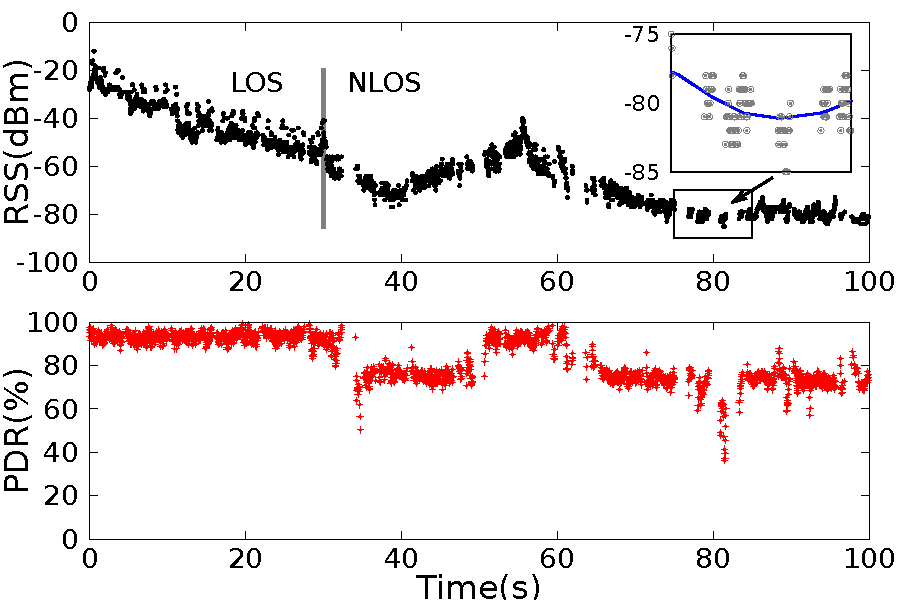
\includegraphics[width=3.2in]{chap2/time.pdf}}
    \hspace{1cm}
    \subfigure[位置差异]{
    \label{fig:cdf_rss}
    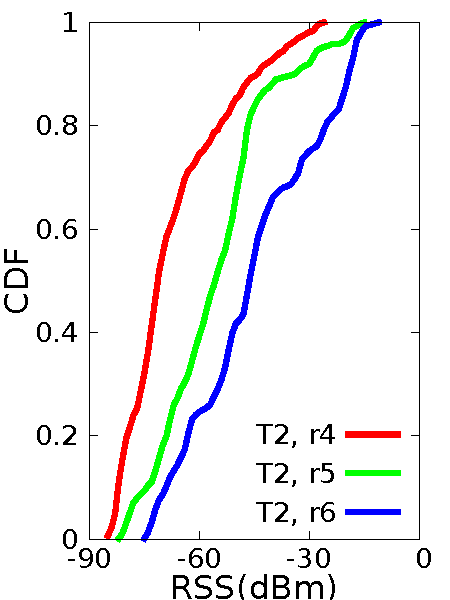
\includegraphics[width=1.6in]{chap2/cdfrss.pdf}}
\bicaption[fig:time]{时变特性与位置差异}{移动网络时变特性及位置差异}{Fig}{Time varying and location difference characteristics of received signal strength}
\end{figure}

The basic consideration in local power estimation is the sampling frequency which is determined by the length of statistical intervals and number of averaging samples. The received signal strength of wireless propagation is influenced by the environments, so the local mean power estimation should be dynamic to the networks status, especially for GSM-R networks. Fig.~\ref{fig:time} demonstrates the time varying and location difference characteristics of received signal strength $P_r(x)$ in mobile networks, which indicates the facts that Fig.~\ref{fig:time_vary}: certain received signal strength carve contains both long-term and short-term fluctuation; Fig.~\ref{fig:cdf_rss}: the overall received signal strength shows different characteristics for different routes. Since the received signal strength $P_r(x)$ is changing in both large and small time scale, the local mean power estimation should also be adaptive to this fluctuation.

A more detailed illustration is given in Fig.~\ref{fig:pdr_over}, which shows the estimation results with different sampling intervals. If the length of averaging interval is set too short, the rapid variations of signal strength will remain in estimation results. This will lead to unstable fluctuation of up-layer decisions, for instance the phenomenon of ping-pong handover when the received signal strength $P_r(x)$ is fluctuating around the threshold. On the other hand, it will lost some crucial information if the statistical interval length is chosen to be too long. As is shown in Fig.~\ref{fig:pdr_over}, the result overestimates the received signal strength when $\Delta t=100$ms, especially when there is sudden decline for received signal strength $P_r(x)$. This overestimation will lead to the decrease of quality of service that the system can provide according to current status.

Lee's method proposed a standard procedure of local average power estimation, which determined the proper length and required sampling numbers for estimating the local average. But Lee's method is conducted in the case of Rayleigh fading channels, which can not be adaptive to environmental changes. The Generalized Lee method allows estimating the mean values without the requirement of a priori knowing the distribution function, which is based on measured field data samples. However the optimum length of averaging interval is calculated using all the routes of the database with high overhead. To make the local mean power estimation adaptive to dynamic prorogation environments with low measurement overhead, the on-line estimation algorithm is proposed which is analyzed in Rician fading channels. The basic process and analysis is presented in detail in the following section.

\section{无线传播模型}
\label{sec:channelmodel}

Since GSM-R networks are deployed along the high-speed railway route with varied terrains, the radio propagation environments are very complex, as is shown in Fig.~\ref{fig:terrain}. It is also obviously in Fig.~\ref{fig:terrain} that the cell radius is normally designed short and the terrain is generally flat, so the multi-path fading should be characterized by Rician fading in this case. There are many Rician channels estimation method such as Training-based Estimation \cite{bjornson2010framework}, Maximum Likelihood \cite{sijbers1998maximum} method, and the Expectation Maximization (EM) algorithm \cite{marzetta1995algorithm}. The EM algorithm provides a complete iterative solution to the Rician parameters estimation in synthetic aperture radar images, which can also be applied in Rician fading channels' parameter estimation.

\begin{figure}[!htp]
\centering
\subfigure[高架]{
    \label{fig:viaduct}
    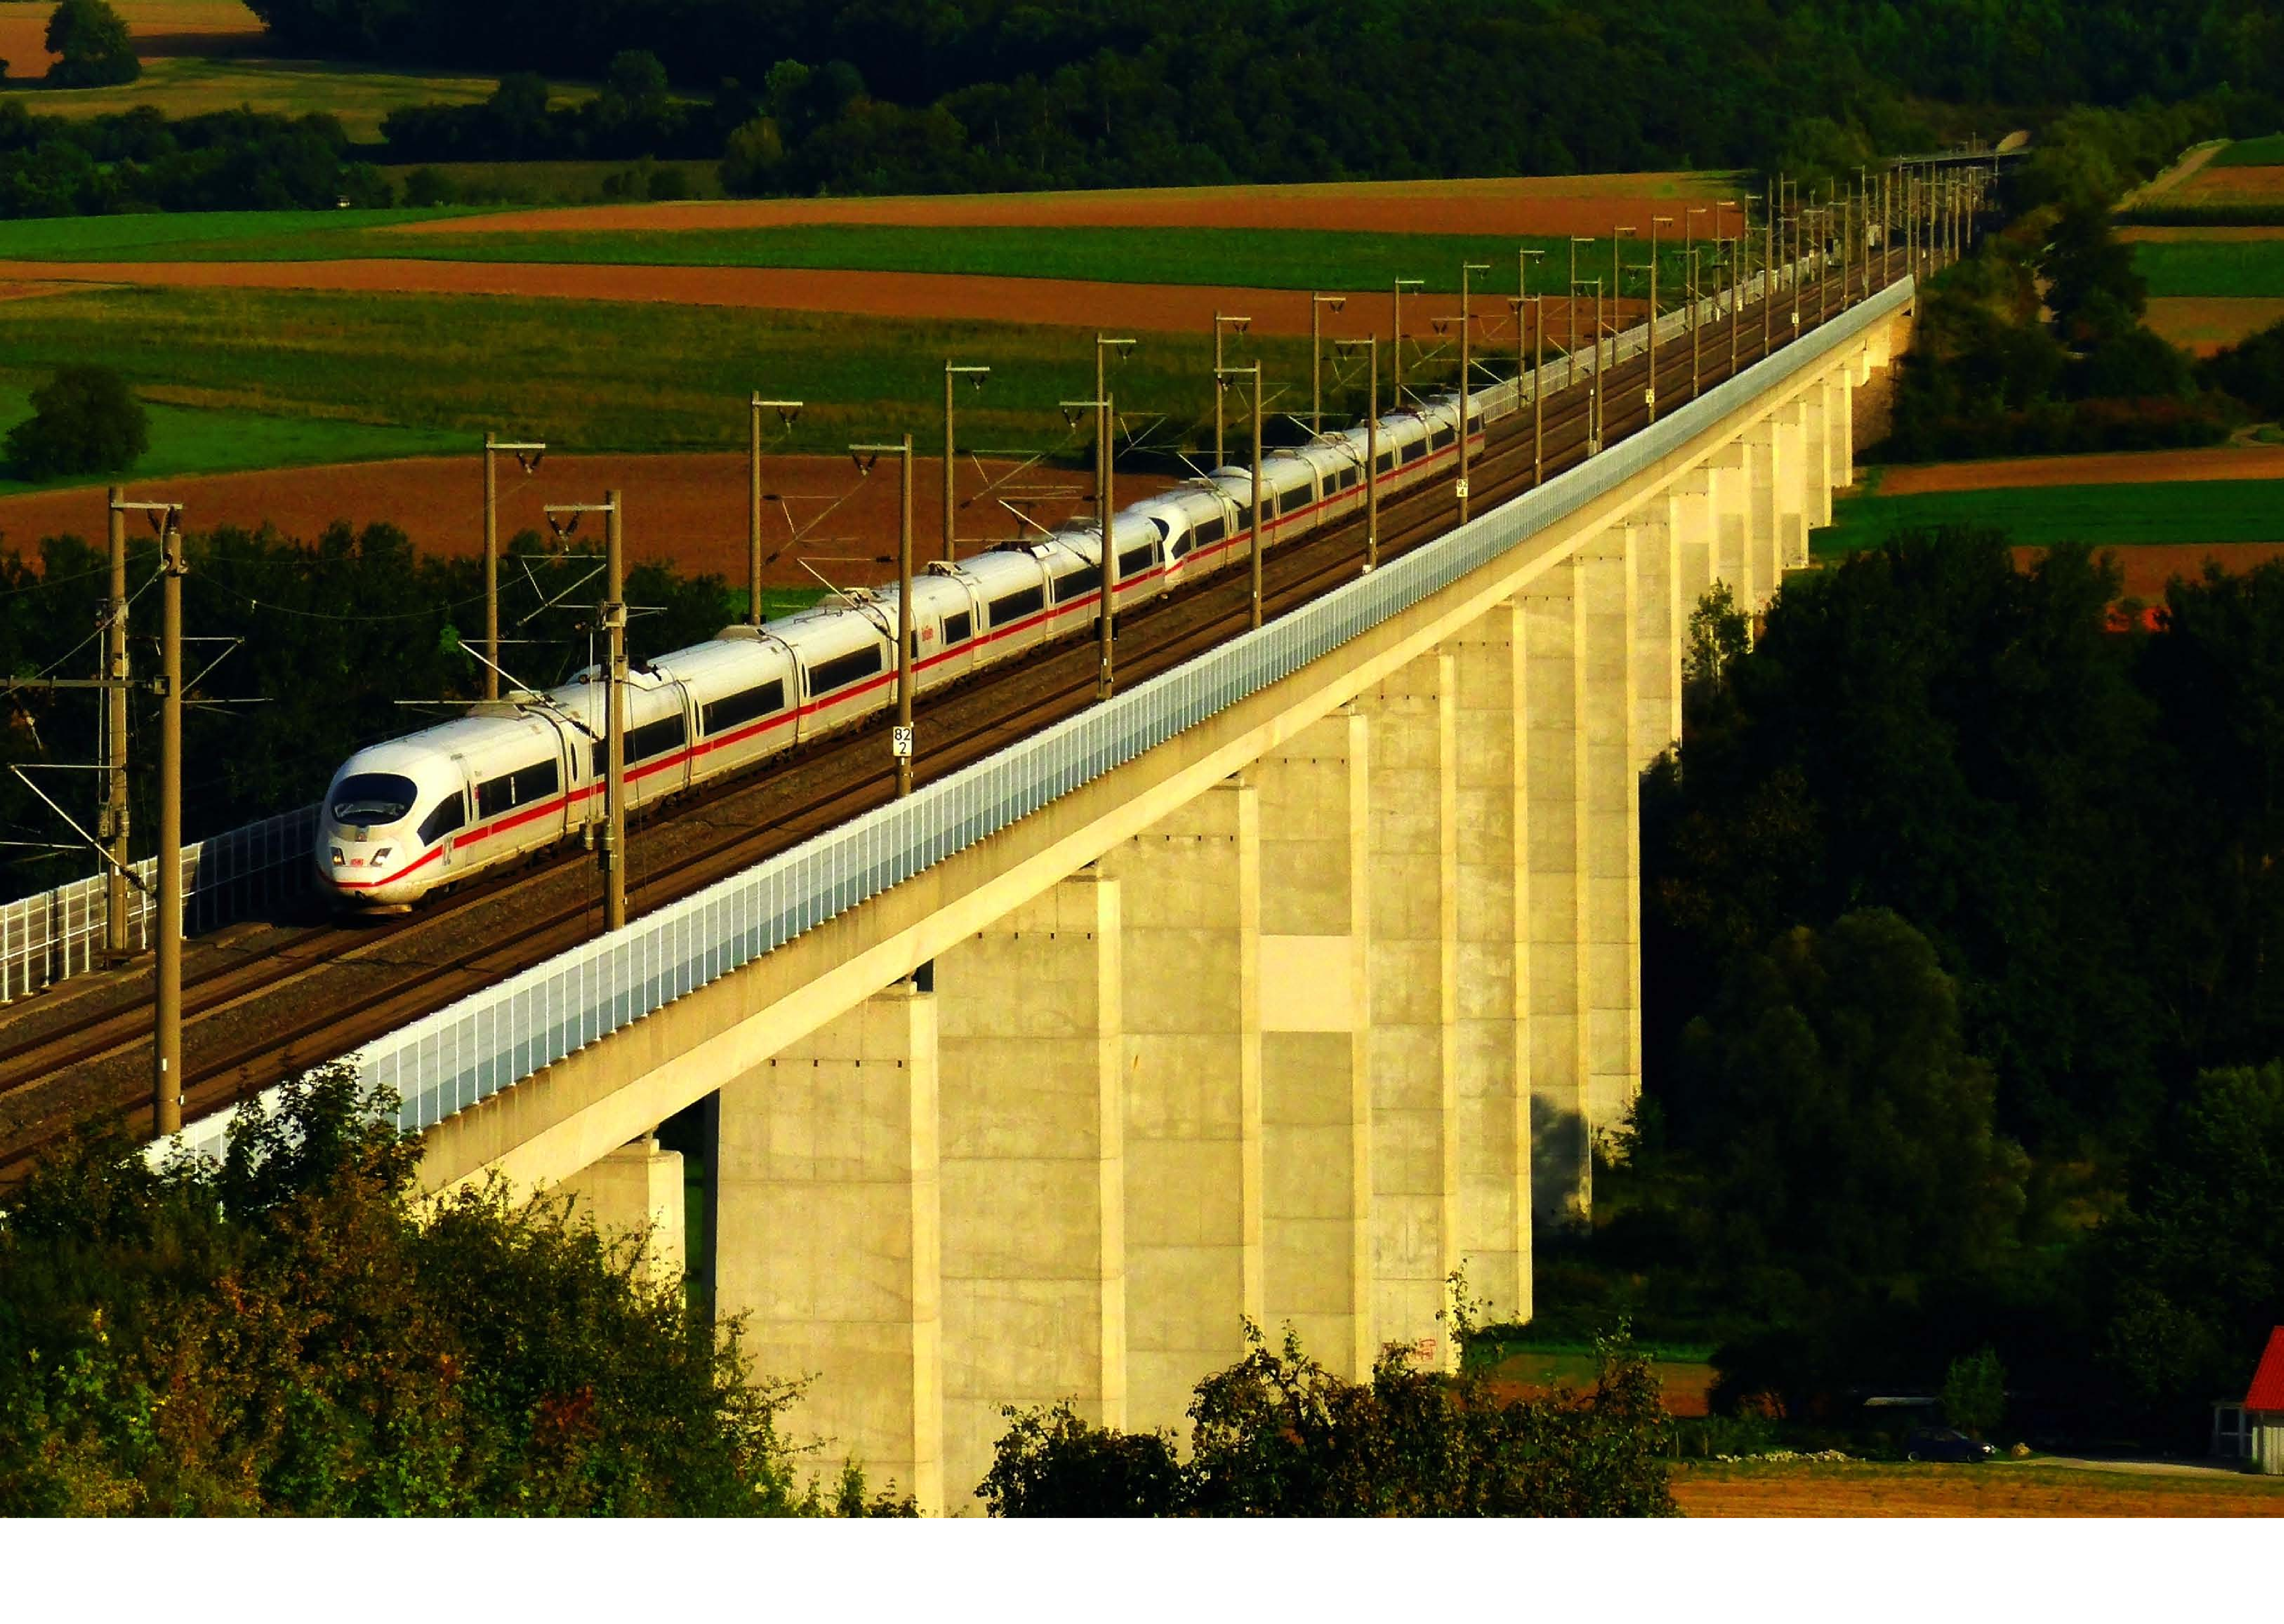
\includegraphics[width=2.5in]{chap2/viaduct.pdf}}
    \hspace{1cm}
\subfigure[隧道]{
    \label{fig:tunnel}
    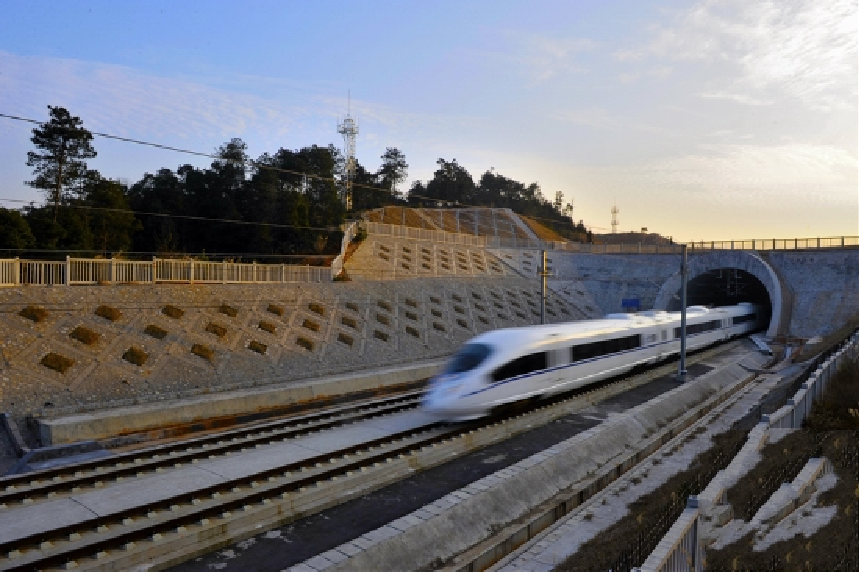
\includegraphics[width=2.5in]{chap2/tunnel.pdf}}
\hspace{1in}
\centering
\subfigure[山区]{
    \label{fig:mountain}
    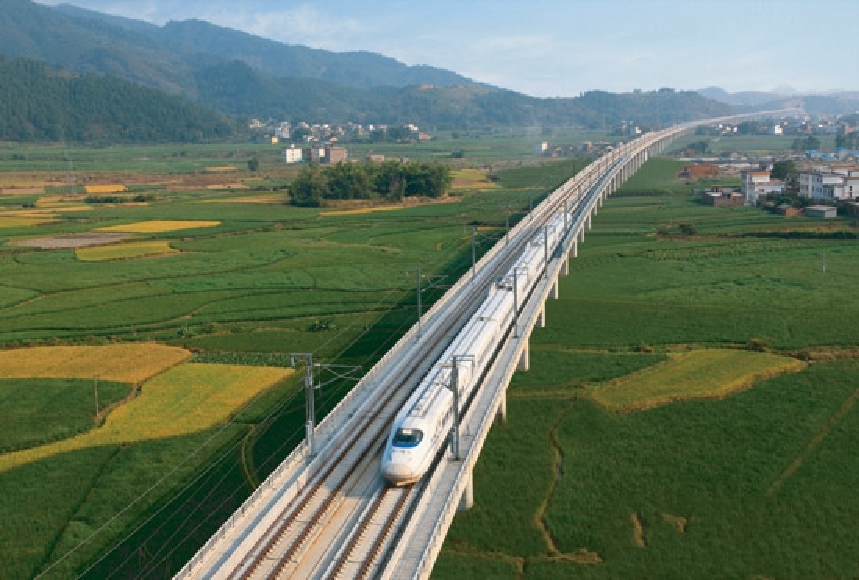
\includegraphics[width=2.5in]{chap2/mountain.pdf}}
    \hspace{1cm}
\subfigure[平原]{
    \label{fig:plain}
    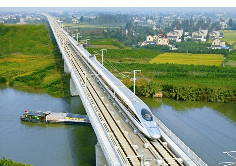
\includegraphics[width=2.5in]{chap2/plain.pdf}}
%\hspace{1in}
%\centering
%\subfigure[车站]{
%    \label{fig:hongqiao}
%    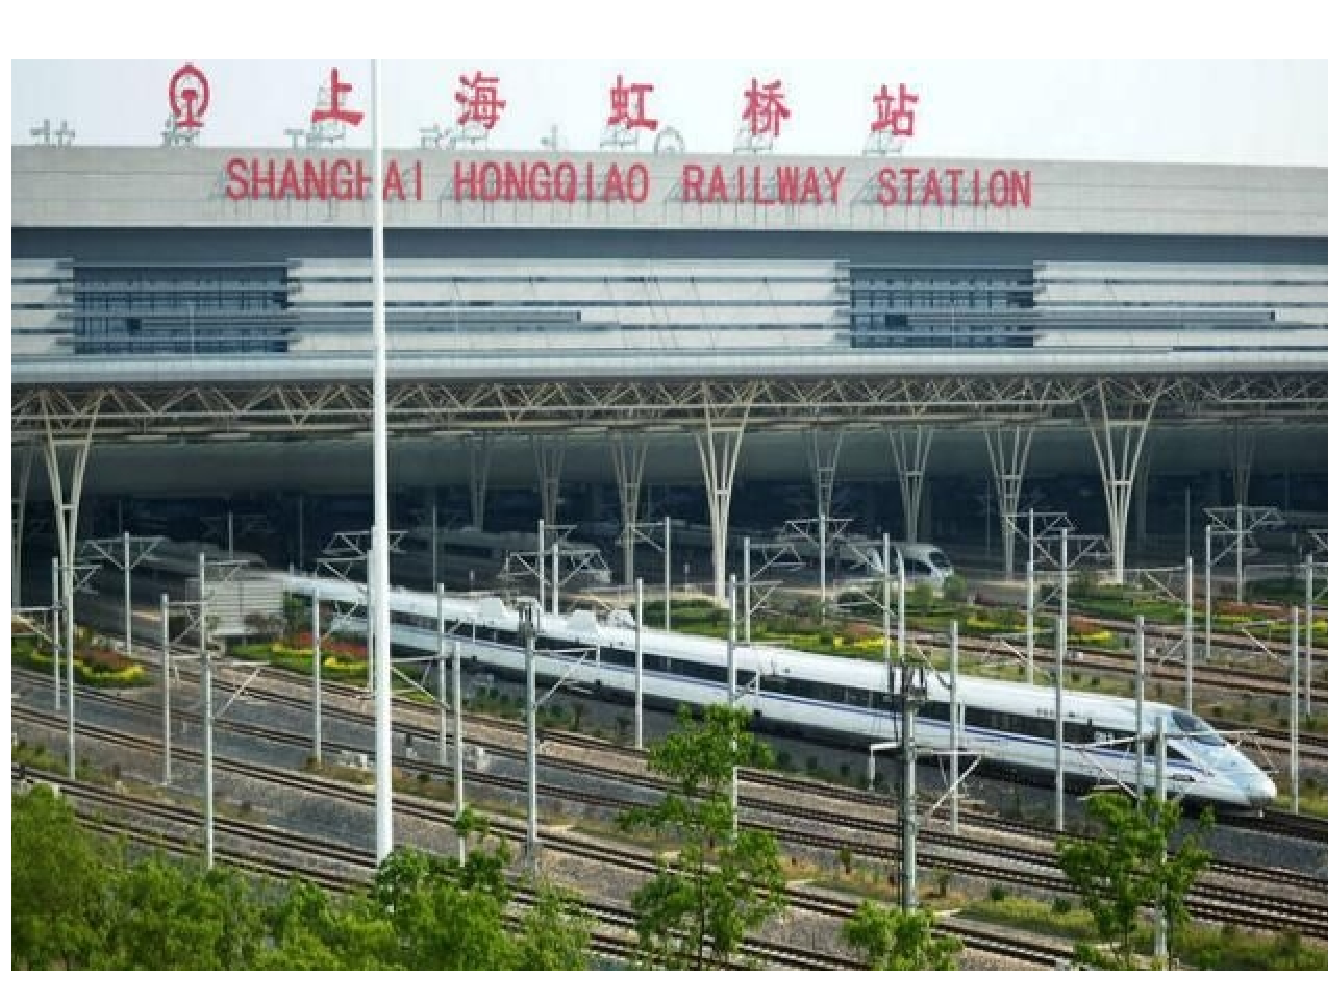
\includegraphics[width=2.5in]{chap2/hongqiao.pdf}}
%    \hspace{1cm}
%\subfigure[基站]{
%    \label{fig:qingzang}
%    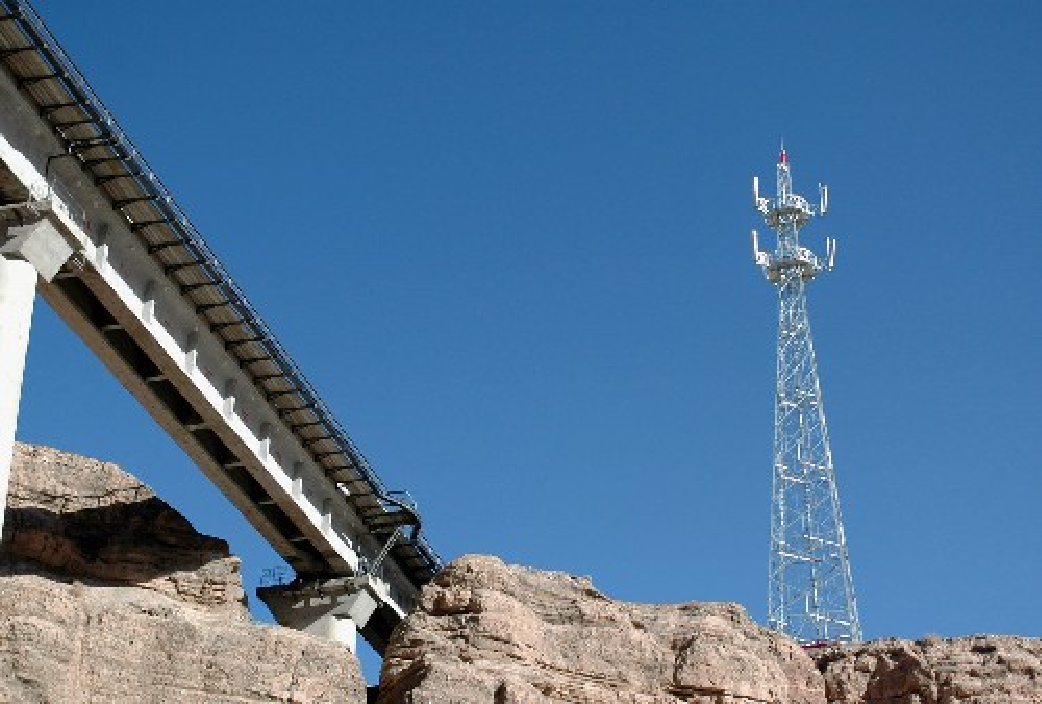
\includegraphics[width=2.5in]{chap2/qingzang.pdf}}
\bicaption[fig:terrain]{GSM-R网络无线传播环境}{GSM-R网络无线传播环境}{Fig}{Radio Propagation Environments and terrains of GSM-R Networks}
\end{figure}

由于高速铁路无线传播环境大多较为平坦,GSM-R网络基站与移动台之间一般存在直射路径,因此高速铁路的无线传播应该以莱斯衰落来刻画。在GSM-R网络空中接口的通信中,接收信号强度可以视为阴影衰落与多径衰落的叠加,如式(3-1)。其中 为阴影衰落,服从高斯过程; 为多径衰落,服从复高斯过程; 可以视为移动台与基站之间距离,利用列车运行速度公式可以转化为时间变量,即 。同时式(3-1)可以表示为对数域形式,如式(3-2)所示,其中 、 、 分别为接收功率与信号衰落在对数域的表示。
\begin{equation}
    p_{r}^{2}(x) = s(x)h(x)
\label{p_r1}
\end{equation}
where $x$ is the distance between MS and BS which can also be replaced by time $t$. Since the distance $d$ between railway track and BS is very short, which is usually about 10m as is shown in Fig.~\ref{train}. Then $\Delta x=\sqrt{d^2+v_{train}^2\cdot \Delta t^2}$ can be deemed as $\Delta x=v_{train}\cdot \Delta t$ by approximation. $p_{r}^{2}(x)$ is the received signal square envelope which is composed of the local mean power $s(x)$ and multi-path fading $h(x)$. The model can also be expressed in logarithmic form as (\ref{P_r2}) in dB values:
\begin{equation}
P_{r}(x) = S(x) + H(x)
\label{P_r2}
\end{equation}
where $P_r(x):=10\log(p_{r}^{2}(x))$, $S(x):=10\log(s(x))$ and $H(x):=10\log(h(x))$.

\begin{figure}[!htp]
\centering
    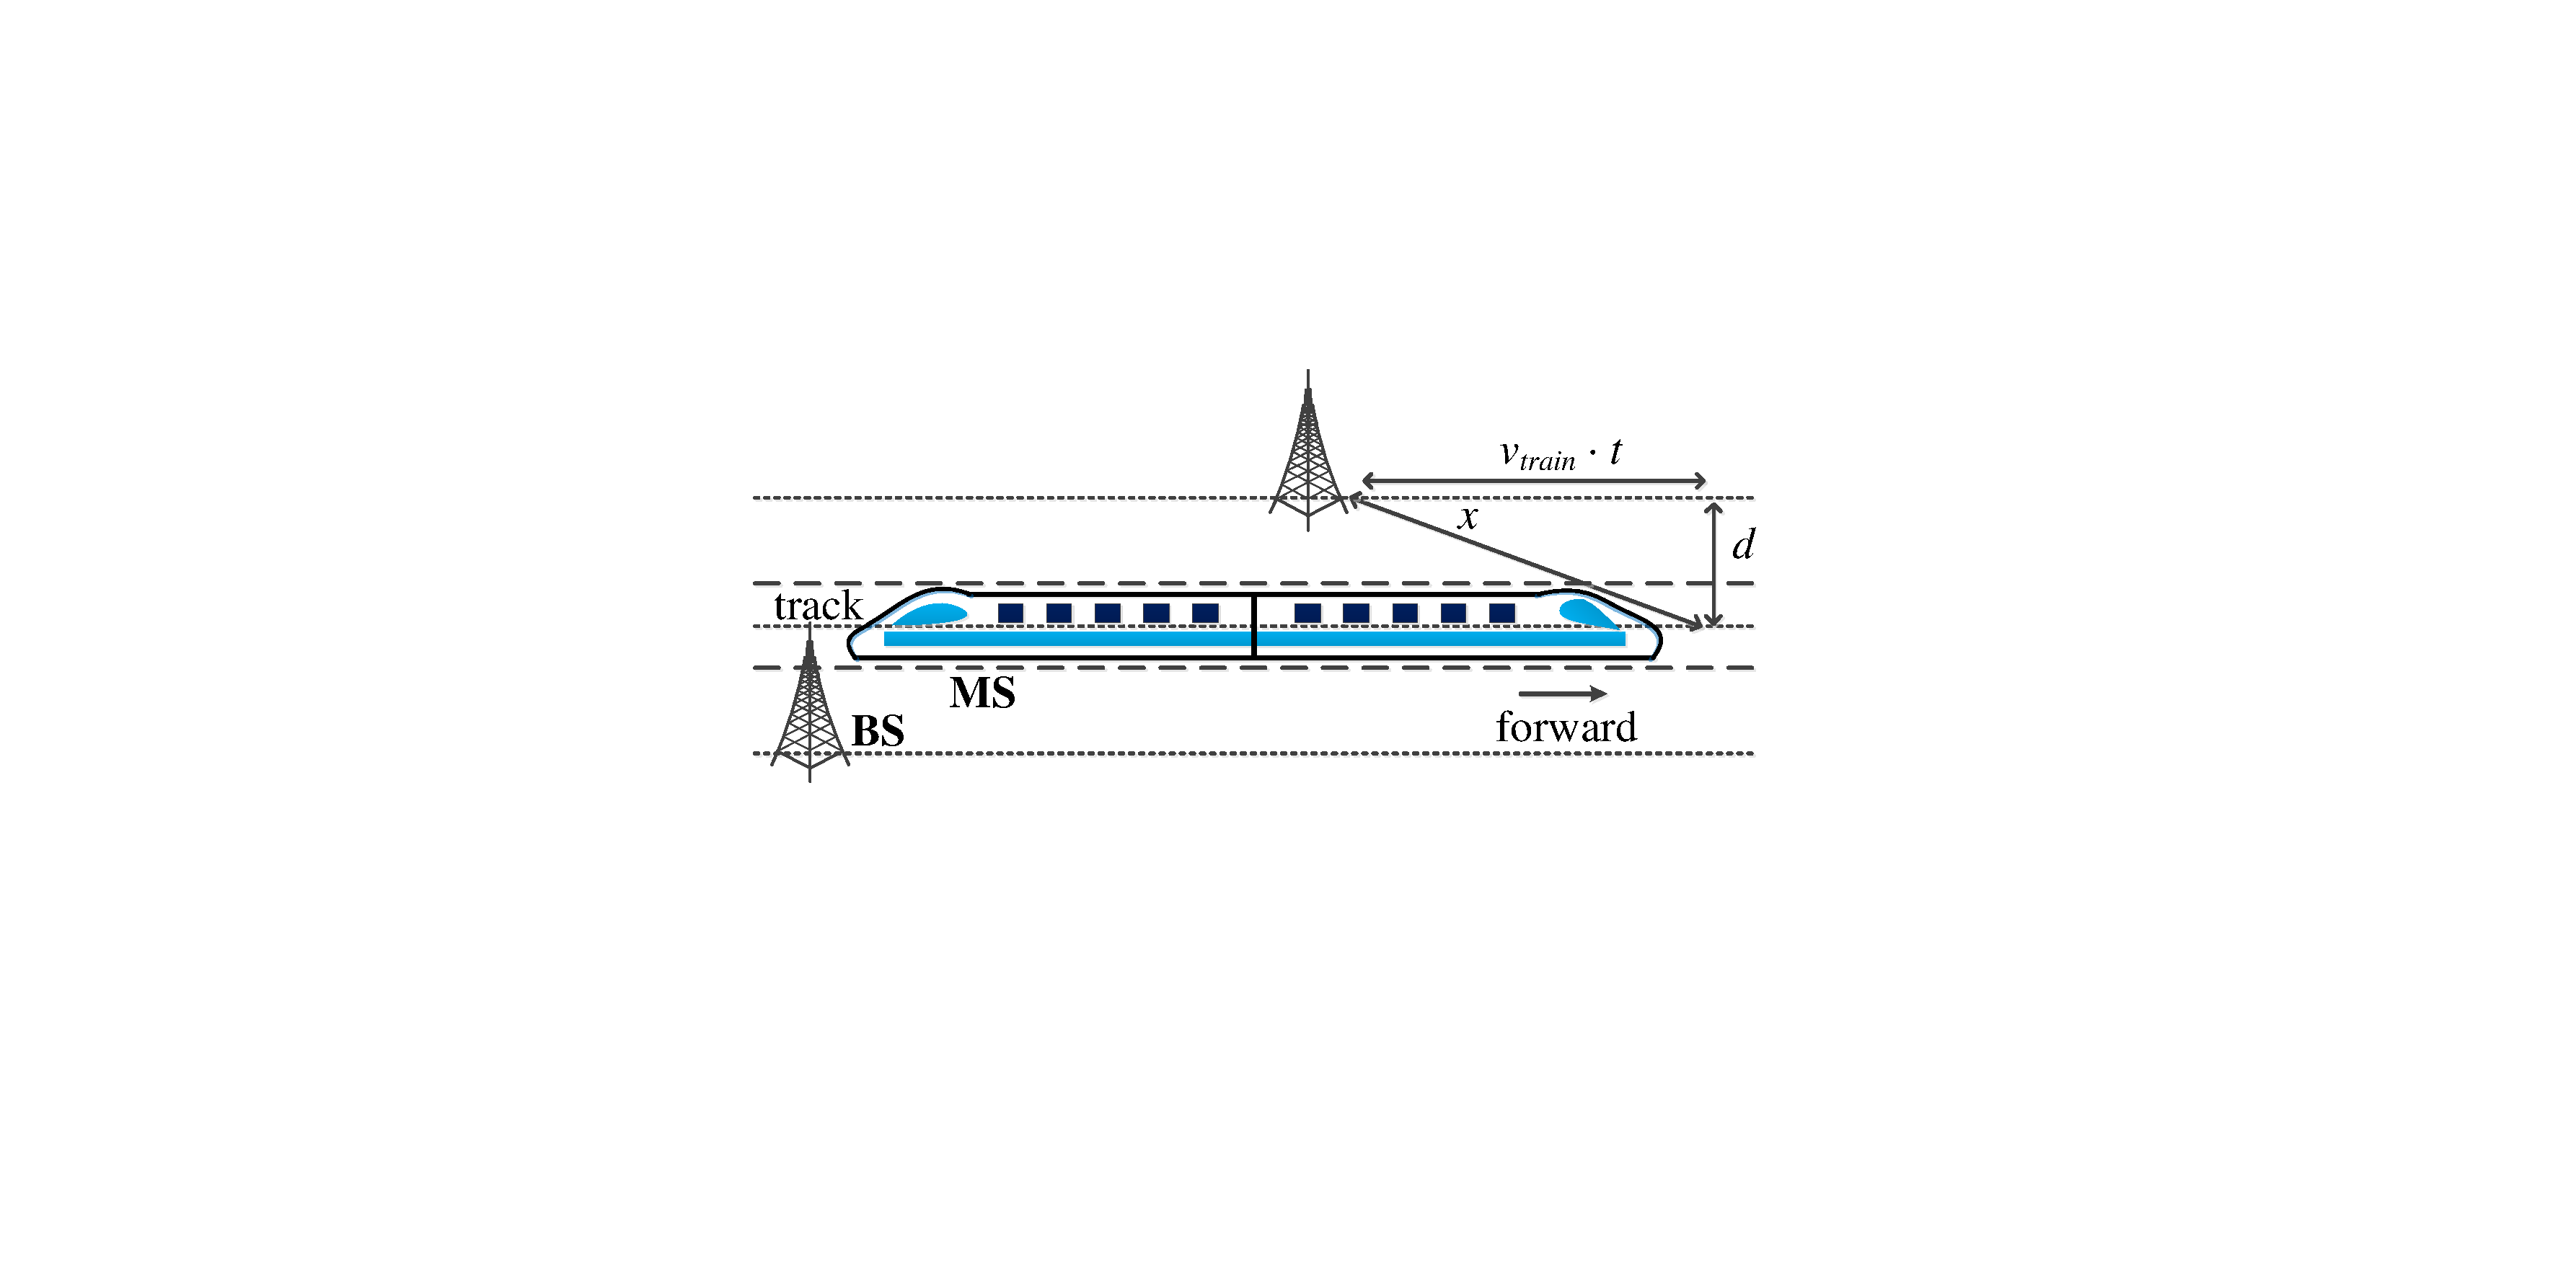
\includegraphics[width=5in]{chap2/train.pdf}
\bicaption[fig:train]{移动台与基站间距离}{移动台与基站间距离}{Fig}{The distance between MS and BS}
\end{figure}

\subsection{阴影衰落}
\label{sec:shadow}

阴影衰落 可用如下的高斯过程表示,其均值 主要受平均路径损耗影响,[20]中给出GSM-R网络平均路径损耗的经验值,可以总结为式(3-4)的形式,其中 反映了基站发射功率大小, 主要受地形因素影响;阴影衰落的方差随着地形的不同而变化,在GSM-R网络中 一般在(3dB,10dB)范围内;参考文献[22]并结合高铁环境,阴影衰落的自相关函数如式(3-5)所示,其中 为阴影衰落方差, 为自相关距离, 为相对距离,可以由列车运行速度及信号采样时间间隔确定,即 。
\begin{equation}
    s(x) \sim N\left( m(x),\sigma_s^2 \right)
\label{shadow}
\end{equation}
where $m(x)$ is mainly affected by path loss. In \cite{sarkar2003survey}, it gives a recommend model comprehensively considering the transmit power of BS, the receive sensitivity of MS, the distance between BS and MS, and the radio propagation environment. The model can be simplified as (\ref{pathloss}).
\begin{equation}
    M(x)= K_1+K_2\log(x)
\label{pathloss}
\end{equation}
where $M(x):=20\log(m(x))$ is the logarithmic form of $m(x)$, $K_1$ denotes the transmit power of BS which both antenna gains and cable losses are taken into account, and $K_2$ is the topographic factor which changes with different terrains\cite{hata1980empirical}\cite{medeisis2000use}. The spatial correlation function of $S(x)$ can be described by (\ref{multipath}) based on measured data in urban and suburban environments\cite{gudmundson1991correlation}.
\begin{equation}
    R_{s}(x) = \sigma_{s}^2\exp\left(-\frac{\Delta x}{x_0}\right)
\label{multipath}
\end{equation}
where $\sigma_s$ is the variance of $S(x)$ which is typically between 4 and 12 dB, $x_0$ is the correlation distance which is normally vary from $10 m$ to $500 m$ in diffident environments\cite{tepedelenlio?lu2001estimation}, and $\Delta x$ is the spatial distance which can be expressed as the velocity of mobile station and the sampling time interval by $\Delta x = v_{train}\cdot\Delta t$. In the model of shadow fading, the topographic factor $K_2$, shadow fading's variance $\sigma_s$ and correlation distance $x_0$ are affected by different terrains, and they are essential to the section of the hysteresis in handoff algorithms. The correlation distance $x_0$ and spatial distance $\Delta x$ affect the optimum estimation accuracy of the local average power.

\subsection{多径衰落}
\label{sec:multipath}

由于GSM-R网络无线传播环境一般较为平坦,存在直射路径,可以认为多径衰落 服从莱斯衰落[23]。式(3-6)为多路径信号的复合叠加,其中 为无线信号波长, 为入射信号与接收天线的夹角, 为各路信号的初始相位。式(3-7)为其概率密度分布,其中 为其它路径与直射路径信号强度的比值,如式(3-8)所示, 为直射路径功率, 为其它路径功率。 为接收信号总功率,表示为直射路径功率 与其它路径功率 的总和,如式(3-9)所示。
\begin{equation}
  h(x)=\underbrace{\frac{1}{\sqrt{1+K}}\lim_{M \to \infty}\frac{1}{\sqrt M}\sum_{m=1}^{M}a_{m}e^{j(\frac{2\pi}{\lambda}\cos(\theta_{m}x)+\phi_m)}}_{\rm NLOS~Components}
  +\underbrace{\sqrt{\frac{K}{1+K}}e^{j(\frac{2\pi}{\lambda}\cos(\theta_{0}x+ \phi_0))}}_{\rm LOS~Component}
\label{rician1}
\end{equation}
%\begin{equation}
%\begin{split}
%  h(x)=&\underbrace{\frac{1}{\sqrt{1+K}}\lim_{M \to \infty}\frac{1}{\sqrt M}\sum_{m=1}^{M}a_{m}e^{j\left(\frac{2\pi}{\lambda}\cos(\theta_{m}x)+\phi_m\right)}}_{\rm NLOS~Components}\\
%  &+\underbrace{\sqrt{\frac{K}{1+K}}e^{j(\frac{2\pi}{\lambda}\cos(\theta_{0}x+ \phi_0))}}_{\rm LOS~Component}
%\end{split}
%\label{rician}
%\end{equation}
where $M$ is the number of independent scatterers, and $\lambda$ is the wavelength. $\theta_m(m=0,1,...M)$ denote the angles between the plane waves and mobile station antenna, and $\phi_m(m=0,1,...M)$ is the phases of each wave component. In Racian fading, the power of LOS and NLOS signals can be described by $\nu^2$ and $2\sigma^2$. $K$ is the ratio between the power in the direct path and the power in the other scattered paths, that is $K=\nu^2/2\sigma^2$. The received signal amplitude is then Rician distributed with parameters $\nu^2$ and $\sigma^2$, and the resulting probability distribution function is:
\begin{equation}
    f(y;\sigma,\nu)=\frac{y}{\sigma^2}e^{-\frac{y^2+\nu^2}{2\sigma^2}}I_0\left(\frac{y\nu}{\sigma^2}\right)
\label{ricianPDF}
\end{equation}
where $I_0(\cdot)$ is the zero-order modified Bessel function of the first kind.
It can be deemed as Rayleigh fading when there is no LOS signal, i.e. $K=0$. In this case, $h(x)$ and the probability distribution function of received signal amplitude can be expressed as:
\begin{equation}
    h(x)=\lim_{M \to \infty}\frac{1}{\sqrt M}\sum_{m=1}^{M}a_{m}e^{j\left(\frac{2\pi}{\lambda}\cos(\theta_{m}x)+\phi_m\right)}
\label{rayleigh}
\end{equation}
\begin{equation}
    f(y;\sigma)=\frac{y}{\sigma^2}e^{-\frac{y^2}{2\sigma^2}}
\label{rayleighPDF}
\end{equation}


\section{信道状态动态估计}
\label{sec:dynamic}

Mark D. Austin在其蜂窝网络的切换算法中对莱斯衰落条件下的采样算法进行了推导[18],得到统计区间与采样点数的近似解,但是该算法过程复杂且计算量较大,无法满足高速移动条件下的信号采样;通用Lee氏采样算法需要对不同的统计区间与采样点数进行验证,因此计算量较大,不符合高铁环境实时测试的要求。
动态测试算法的工作过程如图~\ref{fig:online_measure}所示,首先对信号进行动态采样,得到一组当前时刻的信号强度值,然后经过衰落参数动态估计,得到当前无线传播环境的莱斯衰落参数,然后经过计算得到统计区间与采样点数,同时以此为基础开始下一次信号采样。

\begin{figure}[!htp]
\centering
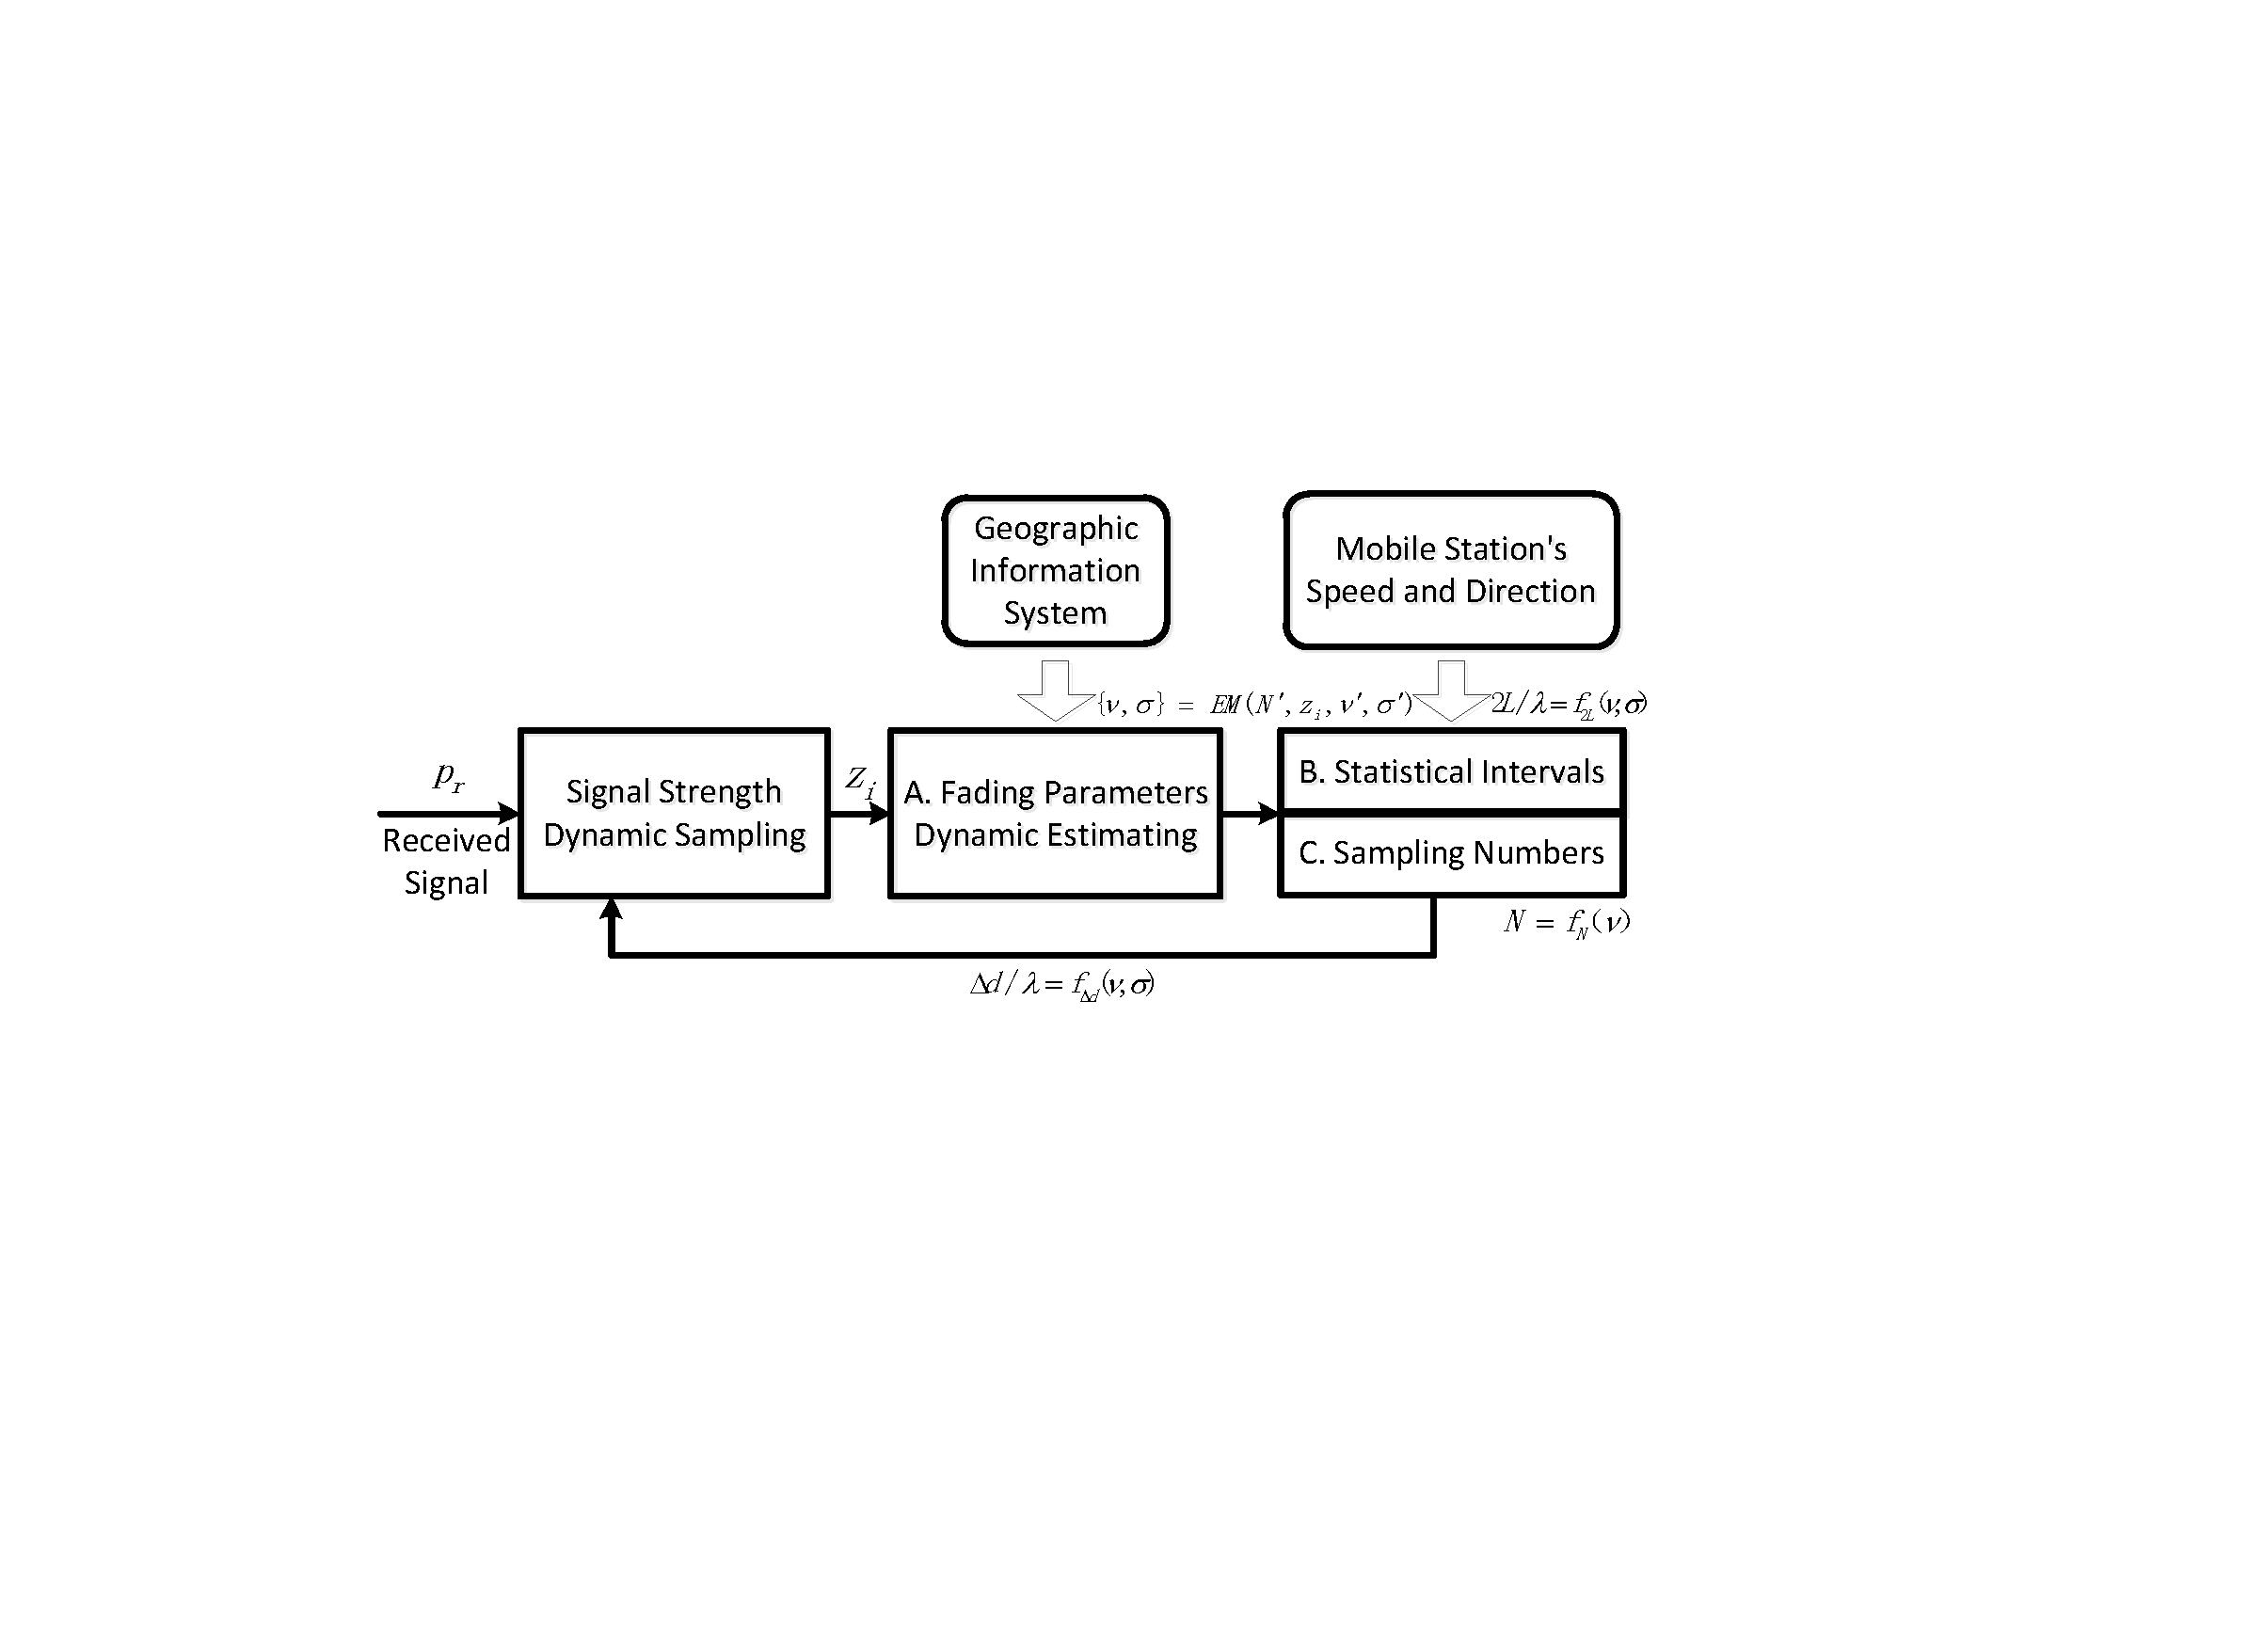
\includegraphics[width=5in]{chap2/online.pdf}
\bicaption[fig:online_measure]{在线动态测试框架}{在线动态测试框架}{Fig}{On-line and Dynamic Estimation of Rician Fading Channels}
\end{figure}

\subsection{信道参数估计}
\label{sec:estimation}

To reduce the estimation overhead, EM algorithm \cite{marzetta1995algorithm} is utilized to estimate the noise variance and the signal simultaneously. The Rician fading parameters $\nu^2$ and $\sigma^2$ are determined by the signal samples and estimation results of last time as follows:
\begin{equation}
    \nu_{k+1}=\frac{1}{N}\sum_{i=1}^{N}\frac{I_{1}\left(\frac{\nu_{k}z_{i}}{\sigma_k^2}\right)}{I_{0}\left(\frac{\nu_{k}z_{i}}{\sigma_k^2}\right)}z_i
\label{EM_nu}
\end{equation}
\begin{equation}
    \sigma_{k+1}^2=\max{\left[\frac{1}{2N}\sum_{i=1}^N z_i^2 -\frac{\nu_k^2}{2},0\right]}
\label{EM_sigma}
\end{equation}
where $I_1(\cdot)$ is is the first-order modified Bessel function of the first kind, $N$ is the number of averaging samples, $\nu_k$ and $\sigma_k$ are the estimation results of last recursion. The initial values are
\begin{equation}
    \nu_{0}=\left(2\left(\frac{1}{N}\sum_{i=1}^N z_i^2\right)^2-\frac{1}{N}\sum_{i=1}^N z_i^4\right)^{1/4}
\label{nu_0}
\end{equation}
\begin{equation}
    \sigma_{0}^2=\frac{1}{2}\left(\frac{1}{N}\sum_{i=1}^N z_i^2 - \nu_{0}\right)
\label{sigma_0}
\end{equation}

Based on the estimated Rician channel parameters, the sampling frequency can be determined, which is in terms with $\lambda$, $\nu$ and $\sigma$. Then the local mean power can be achieved by at least $N$ signal strength samples, which is separated by distance $\Delta d$ within a averaging window of length $2L$.

\subsection{统计区间长度}
\label{sec:length}

The local mean power is estimated by the integration averaging of the sampled signal envelope $p_r(x)$ over a suitable length $2L$. The proper selection of $2L$ should be determined so that the long-term and short-term signals can be separated accurately.

根据Lee氏采样算法,通过接收信号强度求得慢衰落估计值及其方差,慢衰落的估计值为接收信号强度在2L长度的统计区间内的积分平均,计算过程如式(3-19)所示。由文献[20]计算 的方差 ,如式(3-20)所示。

For the propagation models presented in Section \ref{model}, the estimation of $s(x)$ can be calculated by the integral spatial average of $h(x)$ as (\ref{shadow_mean})
\begin{equation}
    \hat{s}=\frac{1}{2L}\int\limits_{y-L}^{y+L} p_r^2(x)dx=\frac{s}{2L}\int\limits_{y-L}^{y+L} h(x)dx
\label{shadow_mean}
\end{equation}

When the $2L$ is properly chosen, the estimated mean $\hat{s}$ will approach the true value $s$, i.e., $\hat{s}\rightarrow s$. At the same time, the averaging of the short-term fading will be
\begin{equation}
\frac{1}{2L}\int\limits_{y-L}^{y+L} h(x)dx \rightarrow 1
\label{short-term}
\end{equation}

According to (\ref{shadow_mean}), the fluctuations of $\hat{s}$ based on $s$ can be evaluated by means of the variance of the estimated value, and the variance of $\hat{s}$ can be calculated by (\ref{shadow_variance}).
\begin{equation}
    \sigma_{\hat{s}}^{2}=\frac{1}{L}\int\limits_{0}^{2L}\left(1-\frac{\tau}{2L}\right)R_{p_{r}^2}(\tau)d\tau
\label{shadow_variance}
\end{equation}
where $R_{p_{r}^2}(\tau)=E[p_{r}^{2}(x)p_{r}^{2}(x+\tau)]-E[p_{r}^{2}(x)]E[p_{r}^{2}(x+\tau)]$ is the autocovariance function of the squared envelope of $p_{r}(x)$. $R_{p_{r}^2}(\tau)$ can be derived from (\ref{rician}) and (\ref{ricianPDF}) by approximation\cite{Austin1994} as follows:
\begin{equation}
    R_{p_{r}^2}(\tau)=4\sigma^2\left[J_0^2\left(\frac{2\pi}{\lambda}\tau\right)+2KJ_0\left(\frac{2\pi}{\lambda}\tau\right)\cos\left(\frac{2\pi}{\lambda}\eta\tau\right)\right]
\label{app:autocovariance}
\end{equation}
where $J_0(\cdot)$ is the zero-order Bessel function, and $\eta=\cos\theta_0$. Then $\sigma_{\hat{s}}^2$ can be calculated by substituting (\ref{app:autocovariance}) into (\ref{shadow_variance}).
%\begin{equation}
%\begin{split}
%\sigma_{\hat{s}}^{2}=&\frac{4\sigma^2}{L}\int\limits_{0}^{2L}(1-\frac{\tau}{2L})\left[J_0^2\left(\frac{2\pi}{\lambda}\tau\right)+2KJ_0\left(\frac{2\pi}{\lambda}\tau\right)\cos\left(\frac{2\pi}{\lambda}\eta\tau\right)\right]d\tau\\
%\stackrel{\rho\triangleq\frac{\tau}{\lambda}}{=}&\frac{\hat{s}^2(2L-\lambda)\lambda}{2(1+K)^{2}L^2}\int\limits_0^{\frac{2L}{\lambda}}\left[J_0^2\left(2\pi \rho\right)+2KJ_0\left(2\pi \rho\right)\cos\left(2\pi \eta\right)\right]\rho d\rho
%\end{split}
%\label{shadow_sigma}
%\end{equation}
\begin{equation}
\begin{split}
\sigma_{\hat{s}}^{2}=&\frac{4\sigma^2}{L}\int\limits_{0}^{2L}\frac{2L-\tau}{2L}[J_0^2(\frac{2\pi}{\lambda}\tau)+2KJ_0(\frac{2\pi}{\lambda}\tau)\cos(\frac{2\pi}{\lambda}\eta\tau)]d\tau\\
=&\frac{\hat{s}^2(2L-\lambda)\lambda}{2(1+K)^{2}L^2}\int\limits_0^{\frac{2L}{\lambda}}[J_0^2(2\pi \rho)+2KJ_0(2\pi \rho)\cos(2\pi \eta)]\rho d\rho
\end{split}
\label{app:shadow_sigma}
\end{equation}
where $\rho=\tau/\lambda$ is the intermediate valuable and $\sigma_{\hat{s}}^2\rightarrow0$ as $2L/\lambda\rightarrow\infty$. $\hat{s}$ can be considered as Gaussian distributed when $2L$ is large enough. Then $\sigma_{\hat{s}}^2$ can be represented by the simple form as follows:
\begin{equation}
\sigma_{\hat{s}}^2=\frac{2(n-1)}{n^2(1+K)^2}\int\limits_0^n g(K;\rho) d\rho
\label{app:sigmareplace}
\end{equation}
where $n:=2L/\lambda$ represents the relationship between statistical intervals $2L$ and wireless prorogation wavelength $\lambda$, $g(K;\rho):=[J_0^2(2\pi \rho)+2KJ_0(2\pi \rho)\cos(2\pi \eta)]\rho$ is the intermediate function. Then the normalized estimation error can be calculated as follows:

\begin{equation}
\begin{split}
P_e:&=10 \log_{10}\left(\frac{\hat{s}+\sigma_{\hat{s}}}{\hat{s}-\sigma_{\hat{s}}}\right) \\
    &=10 \log_{10}\left(\frac{n(1+K)+\sqrt{2(1+n)\int\limits_0^n g(K;\rho) d\rho}}{n(1+K)-\sqrt{2(1+n)\int\limits_0^n g(K;\rho) d\rho}}\right) \\
    &= 10 \log_{10}\left(\frac{\frac{2\sigma^2+\nu^2}{2\sigma^2}n+\sqrt{2(1+n)\int\limits_0^n g\left(\frac{\nu^2}{2\sigma^2};\rho\right) d\rho}}{\frac{2\sigma^2+\nu^2}{2\sigma^2}n-\sqrt{2(1+n)\int\limits_0^n g\left(\frac{\nu^2}{2\sigma^2};\rho\right) d\rho}}\right)
\end{split}
\label{app:Perror}
\end{equation}
where $\nu$ and $\sigma$ are the channel estimation results. The proper length of statistics interval can be obtained in terms with $\nu^2$ and $\sigma^2$ through $P_e=1dB$, i.e., $2L=f_{2L}(\lambda;\nu,\sigma)$ or $2L/\lambda=f_{2L/\lambda}(\nu,\sigma)$, as is shown in Fig.~\ref{fig:length}.

\begin{figure}[!htp]
  \centering
  \subfigure[$\sigma=1$]{
    \label{fig:sigma1}
    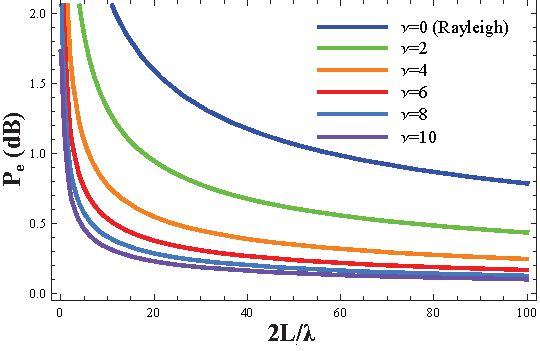
\includegraphics[width=2.5in]{chap2/sigma11.pdf}}
    \hspace{1cm}
  \subfigure[$\sigma=3$]{
    \label{fig:sigma3}
    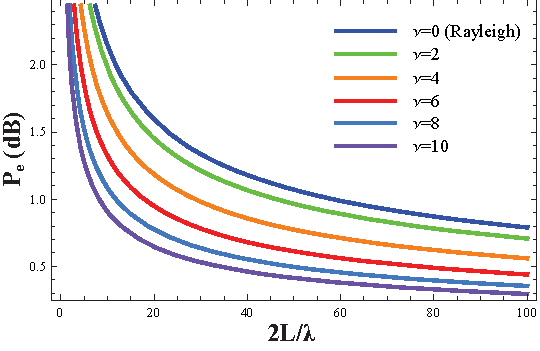
\includegraphics[width=2.5in]{chap2/sigma33.pdf}}
  \hspace{1in}
  \centering
  \subfigure[$\sigma=5$]{
    \label{fig:sigma5}
    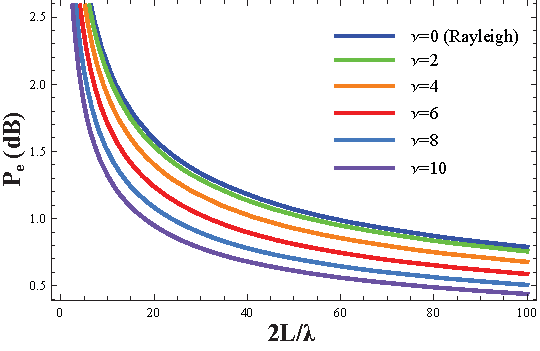
\includegraphics[width=2.5in]{chap2/sigma55.pdf}}
    \hspace{1cm}
  \subfigure[$\sigma=7$]{
    \label{fig:sigma7}
    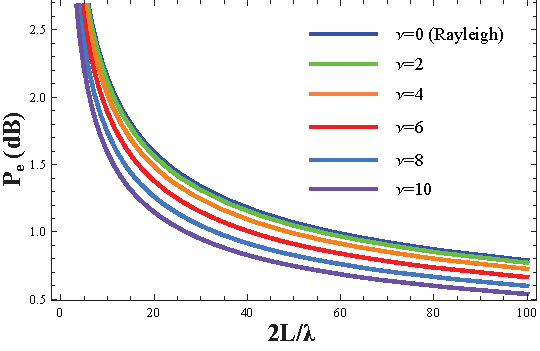
\includegraphics[width=2.5in]{chap2/sigma77.pdf}}
  \bicaption[fig:length]{统计区间长度}{统计区间长度}{Fig}{Proper Length of Statistical Intervals}
\end{figure}

\subsection{采样点数}
\label{sec:number}

Since it needs samples of received signal to sufficiently mitigate the effects of fading, the required number of averaging samples should be determined. The received power can be calculated by $r^2=2\sigma^2+\nu^2\approx\frac{1}{N}\sum_{i=1}^N z_i^2$ through (\ref{EM_nu}) and (\ref{EM_sigma}), and then the expectation and variance of $r^2$ can be calculated:
\begin{equation}
    \bar{r^2}=E\left[r^2\right]=\frac{1}{N}E\left[\sum_{i=1}^{N}z_i^2\right]
\label{number_mean}
\end{equation}
\begin{equation}
    \sigma_{\bar{r^2}}=D\left[r^2\right]=\frac{1}{N^2}D\left[\sum_{i=1}^{N}z_i^2\right]
\label{number_sigma}
\end{equation}

According to the characteristics of Rician distribution, it can be expressed that $z_i^2=x_i^2+y_i^2$ where $x_i \sim N(\nu\cos \eta,\sigma^2)$ and $y_i \sim N(\nu\sin \eta,\sigma^2)$ are statistically independent normal random variables and $\eta$ is any real number. Let $x_{0i}=x_i/\sigma$, then $x_{0i} \sim N(\nu \sin \eta,1)$ and its sum subject to the non-central $\chi^2$ distribution, that is $\sum_{i=1}^{N}x_{0i}^2 \sim \chi_N^2(\nu^2\cos^2\eta)$. For $E[\chi_n^2(\lambda)]=n+\lambda$ and $D[\chi_n^2(\lambda)]=2n+4\lambda$, the mean value and variance of $\sum_{i=1}^{N}x_i^2$ can be calculated by:
\begin{equation}
    E\left[\sum_{i=1}^{N}x_i^2\right]=\sigma^2E\left[\sum_{i=1}^{N}x_{0i}^2\right]=\sigma^2E\left[\chi_N^2(\nu^2\cos^2\eta)\right]=\sigma^2\left(N+\nu^2\cos^2\eta\right)
\label{app:E_x}
\end{equation}
\begin{equation}
    D\left[\sum_{i=1}^{N}x_i^2\right]=\sigma^4D\left[\sum_{i=1}^{N}x_{0i}^2\right]=\sigma^4D\left[\chi_N^2(\nu^2\cos^2\eta)\right]=2\sigma^4\left(N+2\nu^2\cos^2\eta\right)
\label{app:D_x}
\end{equation}
and $E[\sum_{i=1}^{N}y_i^2]=\sigma^2(N+\nu^2\sin^2\eta)$, $D[\sum_{i=1}^{N}y_i^2]=\sigma^4(2N+4\nu^2\sin^2\eta)$ can also be calculated in the same way. Then the expectation of $r^2$ and its variance can be calculated by:
\begin{equation}
\begin{split}
    \bar{r^2}&=E\left[\frac{1}{N}\sum_{i=1}^{N}z_i^2\right]=\frac{1}{N}E\left[\sum_{i=1}^{N}(x_i^2+y_i^2)\right]\\
    &=\frac{\sigma^2}{N}\left(N+\nu^2\cos^2\eta+N+\nu^2\sin^2\eta\right)\\
    &=\frac{\sigma^2}{N}\left(2N+\nu^2\right)
\end{split}
\label{app:E_r2}
\end{equation}
\begin{equation}
\begin{split}
    \sigma_{\bar{r^2}}^2&=D\left[\frac{1}{N}\sum_{i=1}^{N}z_i^2\right]=\frac{1}{N^2}D\left[\sum_{i=1}^{N}\left(x_i^2+y_i^2\right)\right]\\
    &=\frac{\sigma^4}{N^2}\left(2N+4\nu^2\cos^2\eta+2N+4\nu^2\sin^2\eta\right)\\
    &=\frac{\sigma^4}{N^2}\left(4N+4\nu^2\right)
\end{split}
\label{app:D_r2}
\end{equation}

Then the estimation error $Q_e$ can be calculated as follows:
\begin{equation}
\begin{split}
    Q_e&=10 \log_{10}\left(\frac{\bar{r^2}+\sigma_{\bar{r^2}}}{\bar{r^2}}\right)\\
    &=10 \log_{10}\left(\frac{\frac{\sigma^2}{N}\left(2N+\nu^2\right)+\frac{2\sigma^2}{N}\sqrt{N+\nu^2}}{\frac{\sigma^2}{N}(2N+\nu^2)}\right)\\
    &=10 \log_{10}\left(\frac{2N+\nu^2+2\sqrt{N+\nu^2}}{2N+\nu^2}\right)
\end{split}
\label{app:Q_e}
\end{equation}
where $\nu$ and $\sigma$ are the estimation results of EM algorithm in (\ref{EM_nu}) and (\ref{EM_sigma}). Fig.~\ref{nu} gives the relationship between the required number of averaging samples and Rician fading parameter $\nu$, i.e., $N=f_{N}(\nu)$.

The required sampling intervals $\Delta d$ can be easily calculated through $2L/N$, i.e., $\Delta d=f_{2L}(\lambda;\nu,\sigma)/f_{N}(\nu)=f_{\Delta d}(\lambda;\nu,\sigma)$, which can determine the sampling frequency of on-line measurement. Since $\Delta d$ is closely related to the Rician fading parameters $\nu$ and $\sigma$, the Rician factor estimation has a significant influence on the overall measurement efficiency.

The sampling intervals $\Delta d$ has a significant impact on the measurement accuracy and overhead. Note that $\Delta d$ is the ratio of length of statistical interval $2L$ and number of averaging samples $N$, it does not necessarily mean frequent sampling when $2L$ gets short, for $N$ may be very small at the same time.

\begin{figure}[!htp]
\centerline{
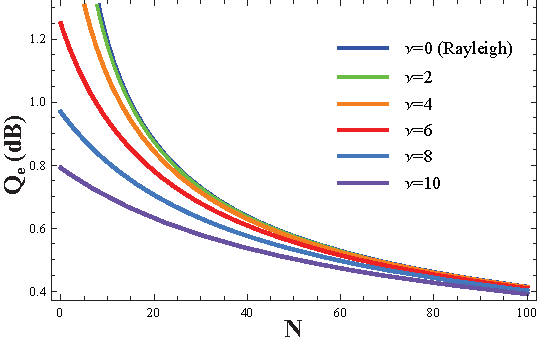
\includegraphics[width=3.0in]{chap2/nu1.pdf}
}
\bicaption[fig:nu]{采样点数}{采样点数}{Fig}{Required Number of Averaging Samples}
\end{figure}


\section{系统实现}
\label{sec:system_phy}

\subsection{GSM-R网络空中接口测试}
\label{sec:um}

The algorithm design and implementation is presented in this section, which first gives a brief description of on-line measurement procedure and then demonstrates the software framework and development.

\begin{algorithm}[!htp]
%\floatname{algorithm}{Procedure}
\renewcommand{\algorithmicrequire}{\textbf{Input:}}
\renewcommand{\algorithmicensure}{\textbf{Output:}}
\caption{On-line estimation of local mean power in Rician fading channels}
\label{alg:online}
\begin{algorithmic}[1]
\Require $v_{train}$, $r_i$, $\nu_k$, $\sigma_k$
\Ensure  $\nu_{k+1}$, $\sigma_{k+1}$, $2L$, $N$, $\Delta d$
\State {// 1. The initialization of $\nu$ and $\sigma$.}
\If {begin-flag==true}
\State {$\Delta d$ $\leftarrow$ Lee($2L_0$,$N_0$;$\lambda$);}
\State {\{$\nu_{last}$, $\sigma_{last}$\} $\leftarrow$ EM($\Delta d$,$N_0$;$r_i$); // Equation(\ref{nu_0}),(\ref{sigma_0})}
\State {\{$\nu_{now}$, $\sigma_{now}$\} $\leftarrow$ EM($\Delta d$,$N_0$;$r_i$;$\nu_{last}$,$\sigma_{last}$); // Equation(\ref{EM_nu}),(\ref{EM_sigma})}
\While {($\nu_{now}-\nu_{last}>\nu_{thr}$) \& ($\sigma_{now}-\sigma_{last}>\sigma_{thr}$)}
\State {\{$\nu_{next}$, $\sigma_{next}$\} $\leftarrow$ EM($\Delta d$,$N_0$;$r_i$;$\nu_{now}$,$\sigma_{now}$); // Equation(\ref{EM_nu}),(\ref{EM_sigma})}
\State {$\{\nu_{last},\sigma_{last}\} \leftarrow \{\nu_{now},\sigma_{now}\}$;}
\State {$\{\nu_{now},\sigma_{now}\} \leftarrow \{\nu_{next},\sigma_{next}\}$;}
\EndWhile
\State {$2L_{now} \leftarrow f_{2L}(\lambda;,\nu_{now},\sigma_{now})$; // Equation(\ref{Perror})}
\State {$N_{now} \leftarrow f_{N}(\nu_{now})$; // Equation(\ref{Qerror})}
\EndIf
\State {// 2. On-line estimation of $\nu$ and $\sigma$, determination of $2L$, $N$ and $\Delta d$.}
\If {operating-flag==true}
\For {$i=0;i<N_{now};i++$}
\State {\{$\nu_{next}$, $\sigma_{next}$\} $\leftarrow$ EM($\Delta d$,$N_0$;$r_i$;$\nu_{now}$,$\sigma_{now}$); // Equation(\ref{EM_nu}),(\ref{EM_sigma})}
\State {$2L_{next} \leftarrow f_{2L}(\lambda;,\nu_{now},\sigma_{now})$; // Equation(\ref{Perror})}
\State {$N_{next} \leftarrow f_{N}(\nu_{now})$; // Equation(\ref{Qerror})}
\State {$\Delta d_{next} = f_{2L}(\lambda;,\nu_{now},\sigma_{now})/f_{N}(\nu_{now})$;}
\State {$\{\nu_{last},\sigma_{last};2L_{last},N_{last}\} \leftarrow \{\nu_{now},\sigma_{now};2L_{now},N_{now}\}$;}
\State {$\{\nu_{now},\sigma_{now};2L_{now},N_{now}\} \leftarrow \{\nu_{next},\sigma_{next};2L_{next},N_{next}\}$;}
\If {$i==N_{last}$}
\State {i=0;}
\EndIf
\EndFor
\EndIf
\end{algorithmic}
\end{algorithm}

The on-line estimation algorithm is given in Algorithm~\ref{alg:online}, which is based on the derivation and calculation introduced in the previous section. First, the initialization is conducted to calculate the initial value of Rician fading factors $\nu_0$ and $\sigma_0$. It is calculated by EM algorithm with the statistical interval length $2L=40\lambda$ and averaging sample numbers $N=36$. Then $\nu_k$ and $\sigma_k$ are estimated in every $k$-th compute cycle based on the estimation results of the last round. At the same time, the averaging factors $2L$ and $N$ of next cycle are calculated based on the measurement samples and Rician fading factors. Finally, the sampling interval is determined by $\Delta d=2L/N$, which can be converted to the time scale by the current velocity of train $v_{train}$. The process of received signal strength sampling and fading channels factors estimation is conducted in each compute cycle.

\begin{figure}[!htp]
%\onelinecaptionsfalse
\centering
    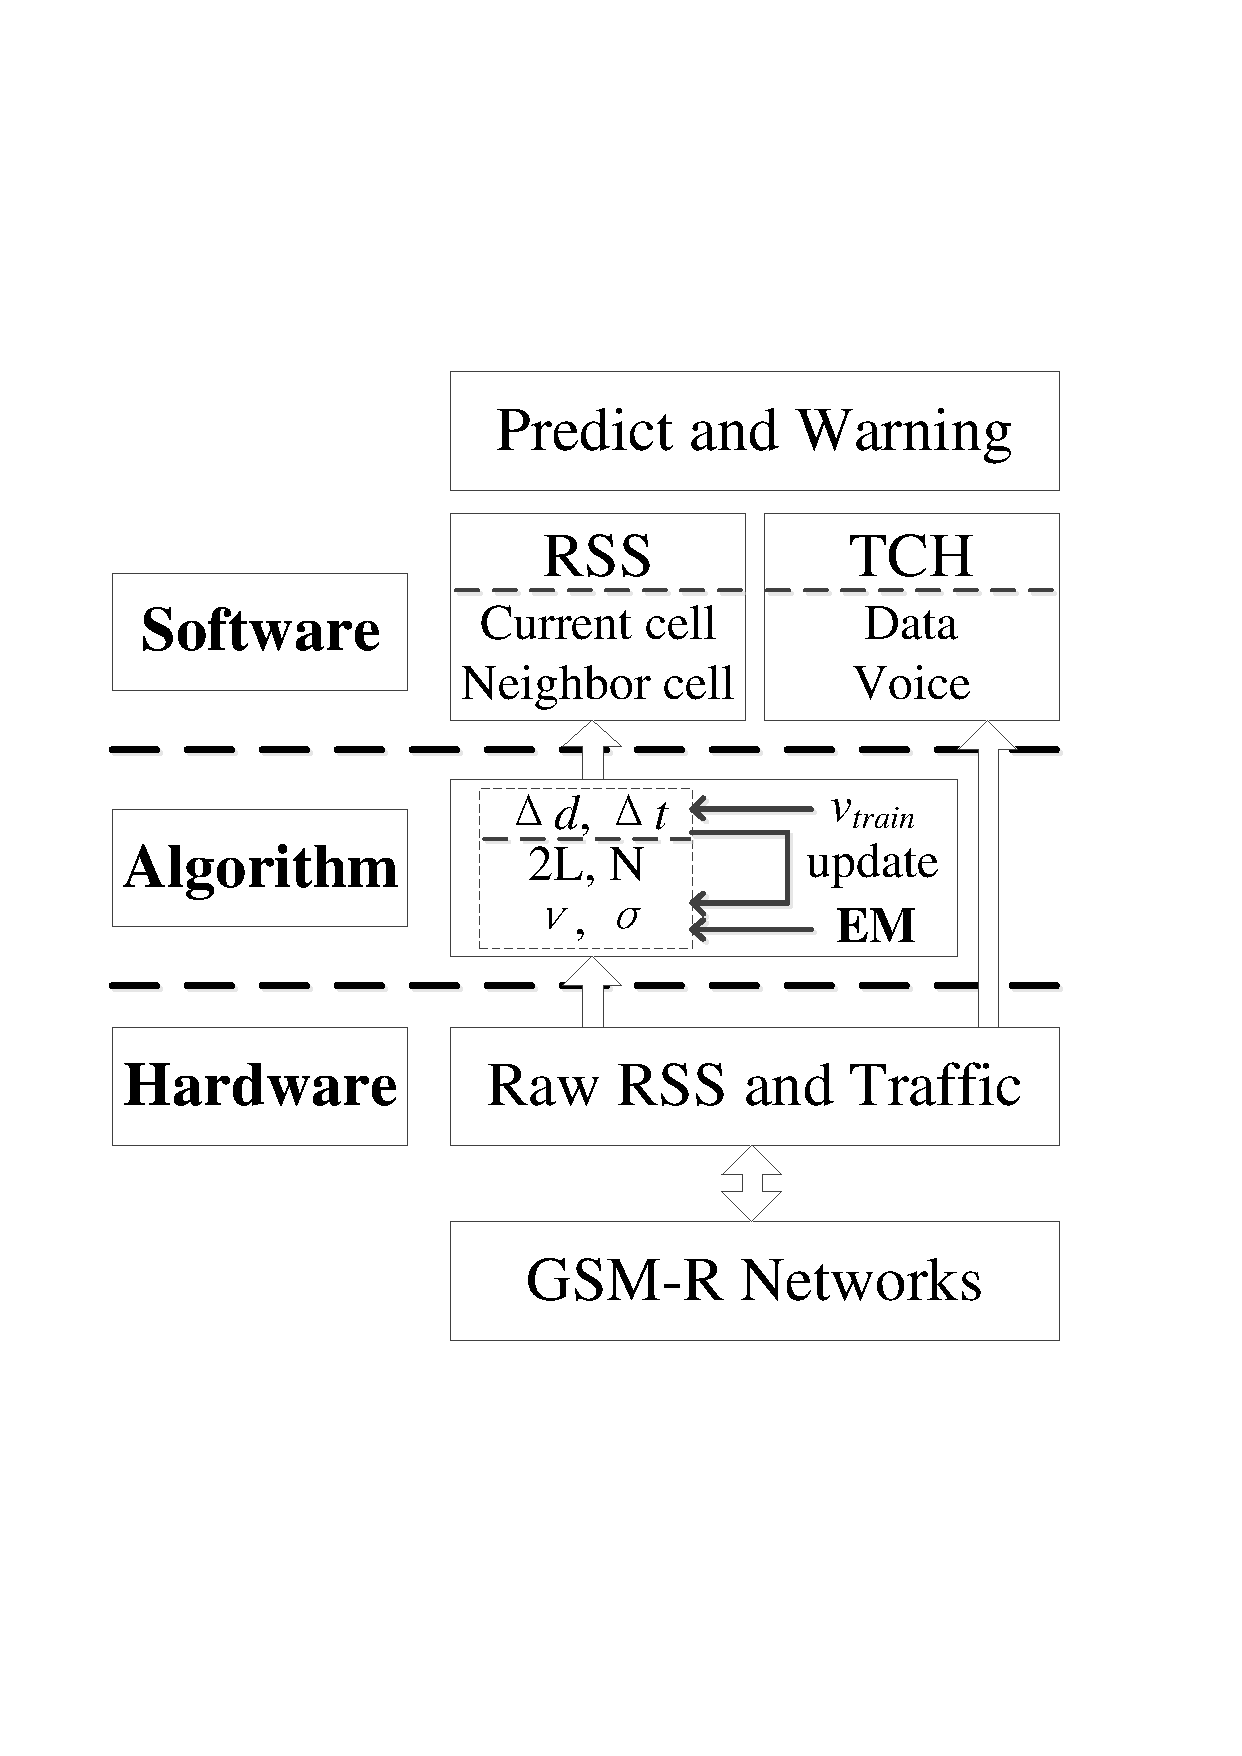
\includegraphics[width=4in]{chap2/umframework.pdf}
\bicaption[fig:umframework]{信道状态估计算法与实现}{信道状态估计算法与实现}{Fig}{Estimation framework and algorithm implementation}
\end{figure}

To get the received data and evaluate the measurement performance, we developed the Um interface monitoring system for GSM-R networks. The hardware and software architecture is shown in Fig.~\ref{fig:platform}, and the online estimation algorithm is implemented on this platform. The system's cpu module is RTD's CME137686LX-W including a 333MHz AMD Geode LX processor with 128kB L1 cache and 128kB L2 cache, and the communication module is COM16155RER-1 using Triorail's GSM-R engine TRM:3a. The system's power supply, processor and comunication module are connected through PC/104 bus, and other peripherals through its specific interface. The hardware components is demonstrated in Fig.~\ref{fig:hardware}. The software is independently developed by our research group, which uses Microsoft .NET Compact Framework in C\#, and it can run on various operating systems including Windows XP, Windows Mobile, and Windows CE. The software interface is shown in Fig.~\ref{fig:software}.

\begin{figure}[!htp]
\centering
\subfigure[Hardware Design]{
    \label{fig:hardware}
    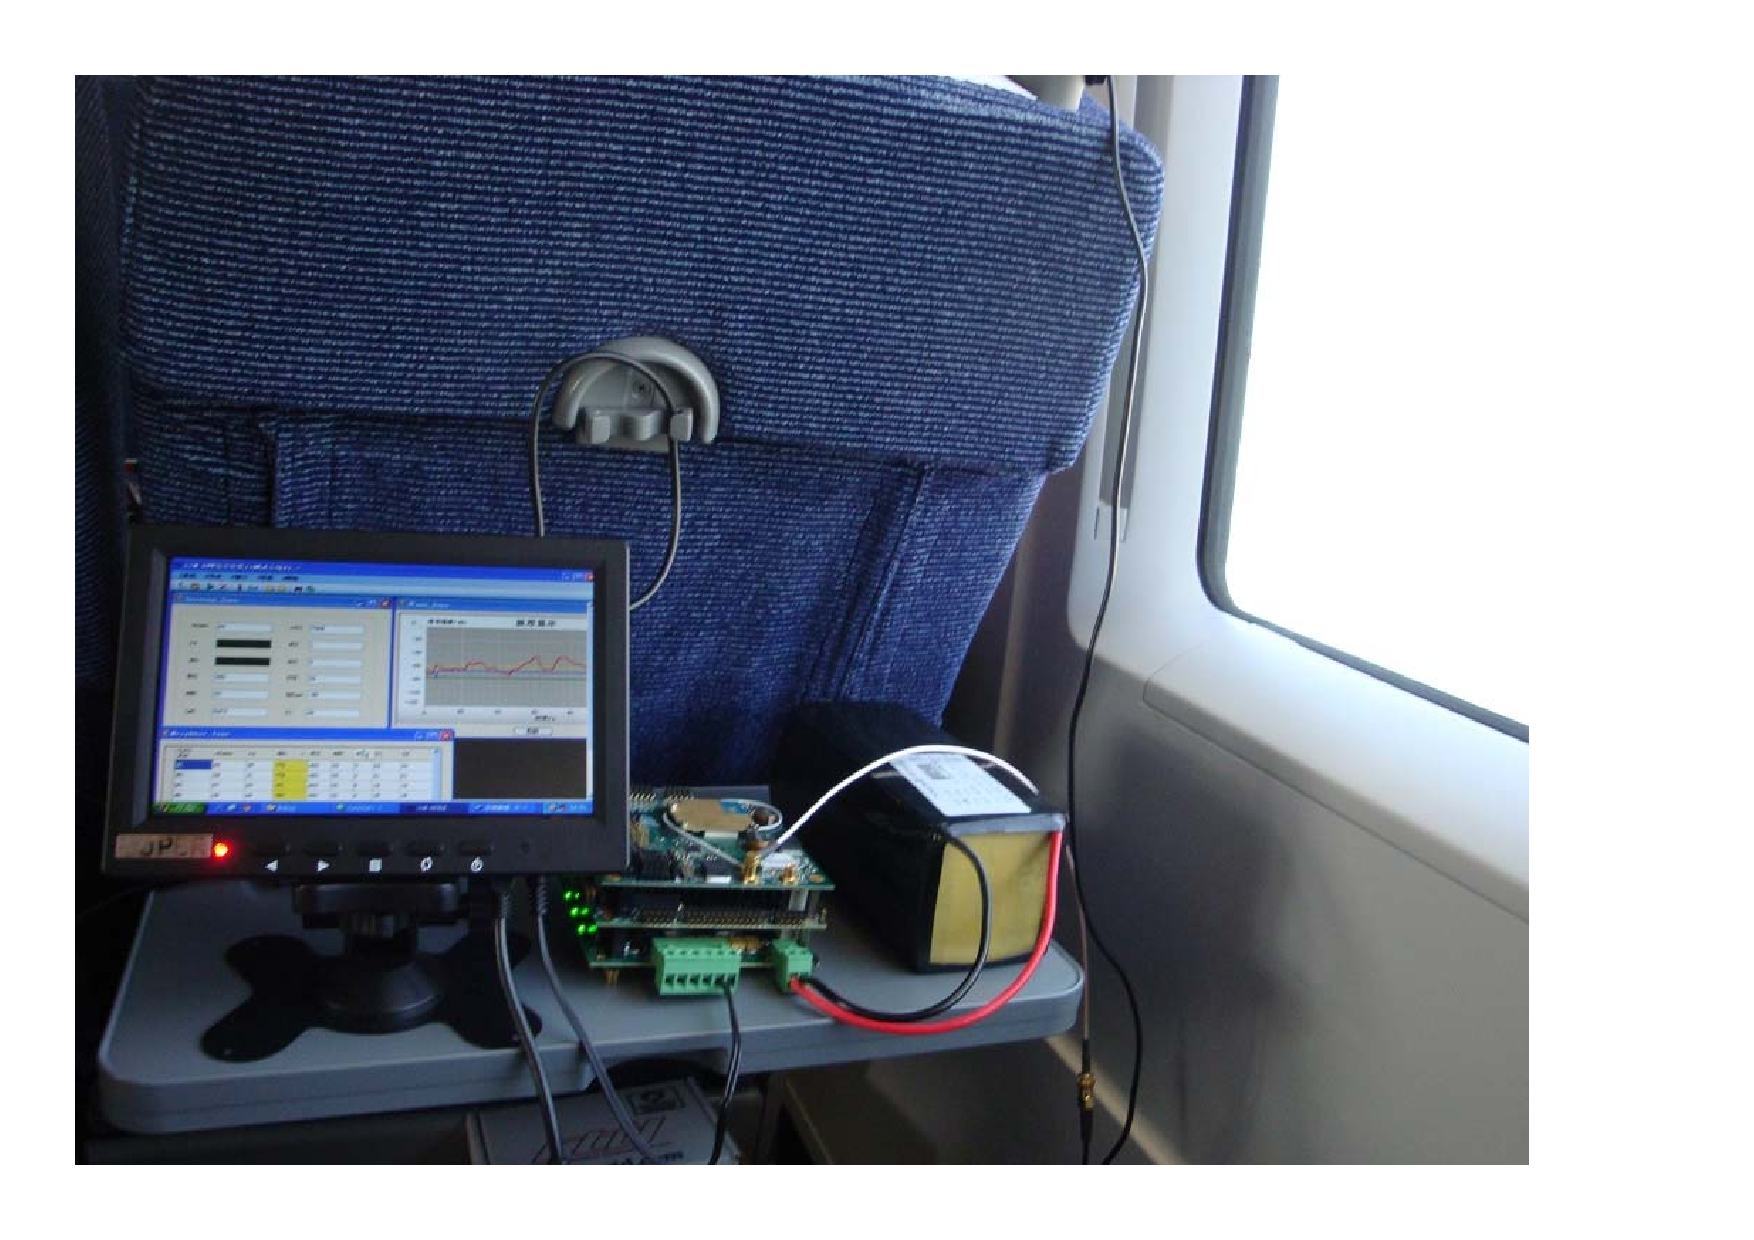
\includegraphics[width=2.5in]{chap2/platform.pdf}}
    \hspace{1cm}
\subfigure[Software Development]{
    \label{fig:software}
    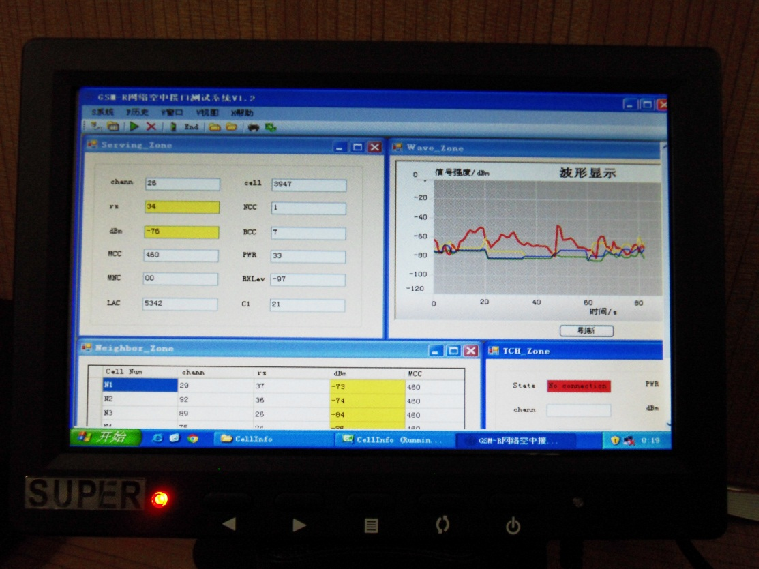
\includegraphics[width=2.5in]{chap2/softwareinterface.pdf}}
\bicaption[fig:platform]{GSM-R网络空中接口测试系统}{GSM-R网络空中接口测试系统}{Fig}{Um Interface Monitoring System for GSM-R Networks}
\end{figure}

As is illustrated in Fig.~\ref{fig:umframework}, the on-line estimation algorithm provides basic information to up-layer applications. The raw data of received signal strength is collected by GSM-R device, which is composed of the information of current cell and 6 neighbour cells. Then these data is processed by the on-line estimation algorithm to provide current network status and conduct next signal sampling. The system also provides received signal strength prediction based on the weighted averaging of signal samples, and gives warning information when the communication performance is lower than certain threshold. Since the system records the received signal strength of current and neighbour cells, the data can be used to make handover analysis and network optimization. Except the physical layer information, the system can also give quality of service of the link layer, including data traffic and voice service.


\section{性能评估}
\label{chap:evaluation_phy}

\subsection{接收信号强度}
\label{sec:rss}

This section presents the experiment and evaluation of on-line and dynamic estimation algorithm proposed previously. Received signal strength measurements, which is implemented by GSM-R network monitoring system, were carried out along the Beijing-Shanghai high-speed railway, and the accuracy and overhead of the algorithm is evaluated in the following.

The measurement experiment is carried out by the Um interface monitoring system of GSM-R networks, as is shown in Fig.~\ref{fig:platform}. The received signal strength was collected along the Beijing-Shanghai high-speed railway, as is shown in Fig.~\ref{fig:experiment}. Since the velocity of train is up to 300km/h and the sampling interval is 500ms limited by the length of measurement multi-frame, it requires repeated data collection to evaluate the estimation algorithm.

%\begin{figure}[!htp]
%%\onelinecaptionsfalse
%\centering
%    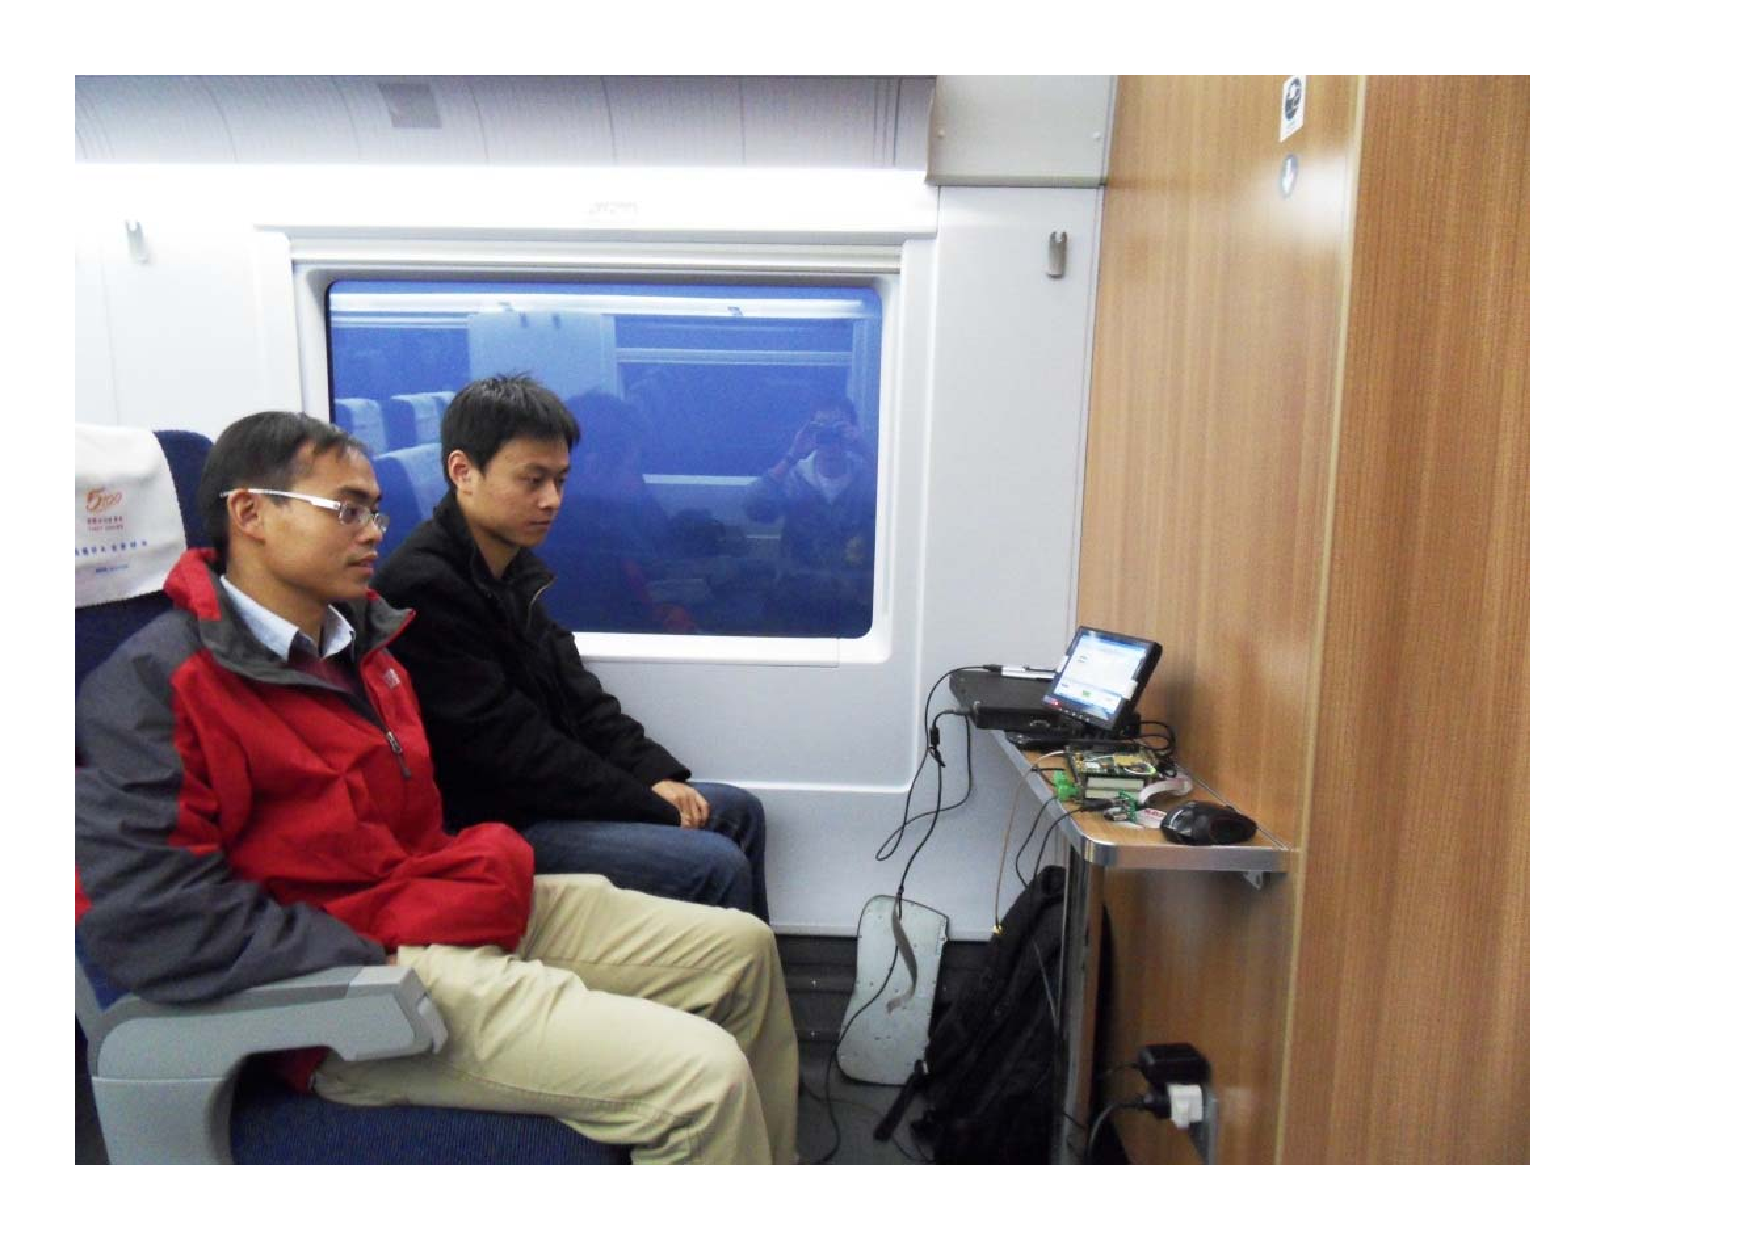
\includegraphics[width=4in]{chap6/test.pdf}
%\bicaption[fig:experiment]{京沪高铁实验测试}{京沪高铁实验测试}{Fig}{Experiment along the Beijing-Shanghai High-Speed Railway}
%\end{figure}

The measurement results is demonstrated in Fig.~\ref{fig:input}, and the long-term and short-term fading are separated after on-line propagation estimation. As is shown in Fig.~\ref{fig:output}, the long-term and short-term fading are differentiated so that they can be analyzed separately. The long-term parts can be used to make propagation prediction by Maximum Likelihood (ML) or Minimum Mean Square Error (MMSE) estimator. On the other hand, the short-term variations are essential to the section of the hysteresis in handoff algorithms.

\begin{figure}[!htp]
\centering
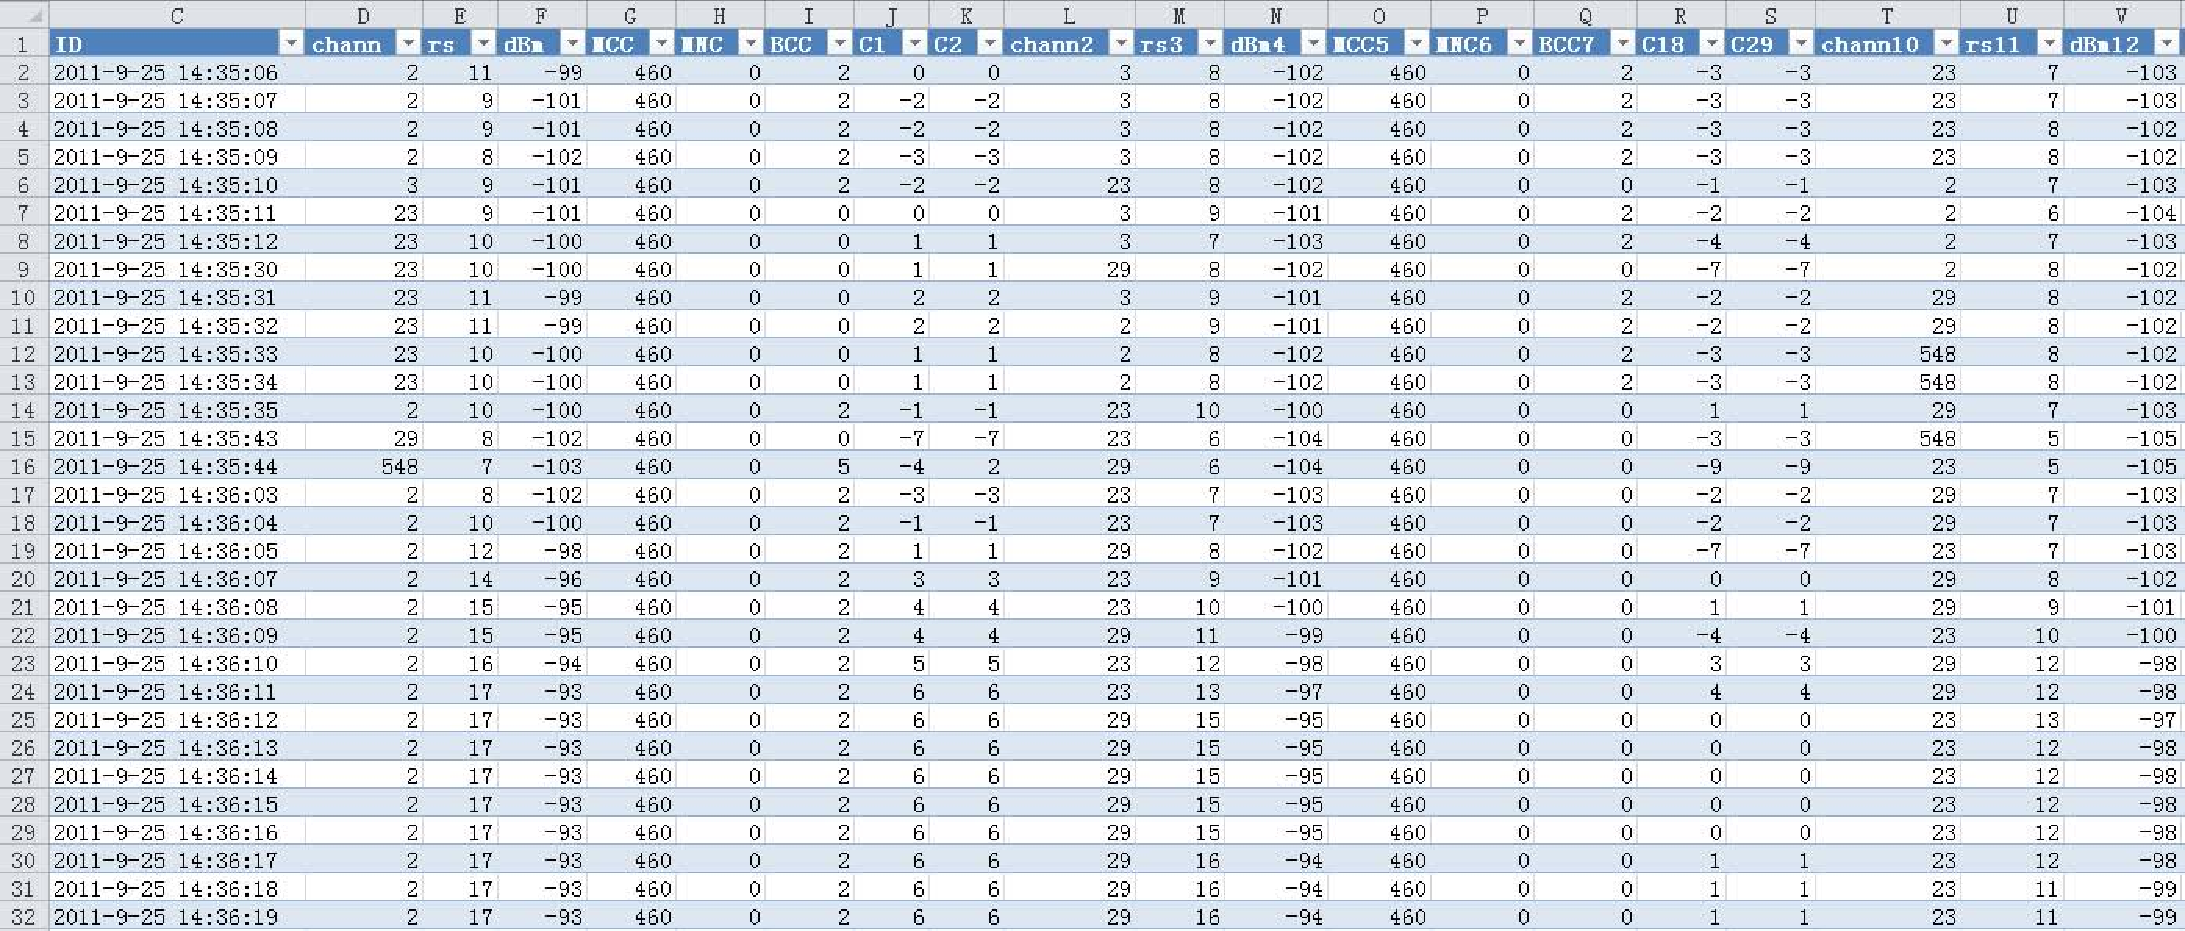
\includegraphics[width=5in]{chap2/xml.pdf}
\bicaption[fig:xml]{信道状态测试结果}{信道状态测试结果}{Fig}{Measurement Results}
\end{figure}

\begin{figure}[!htp]
\centering
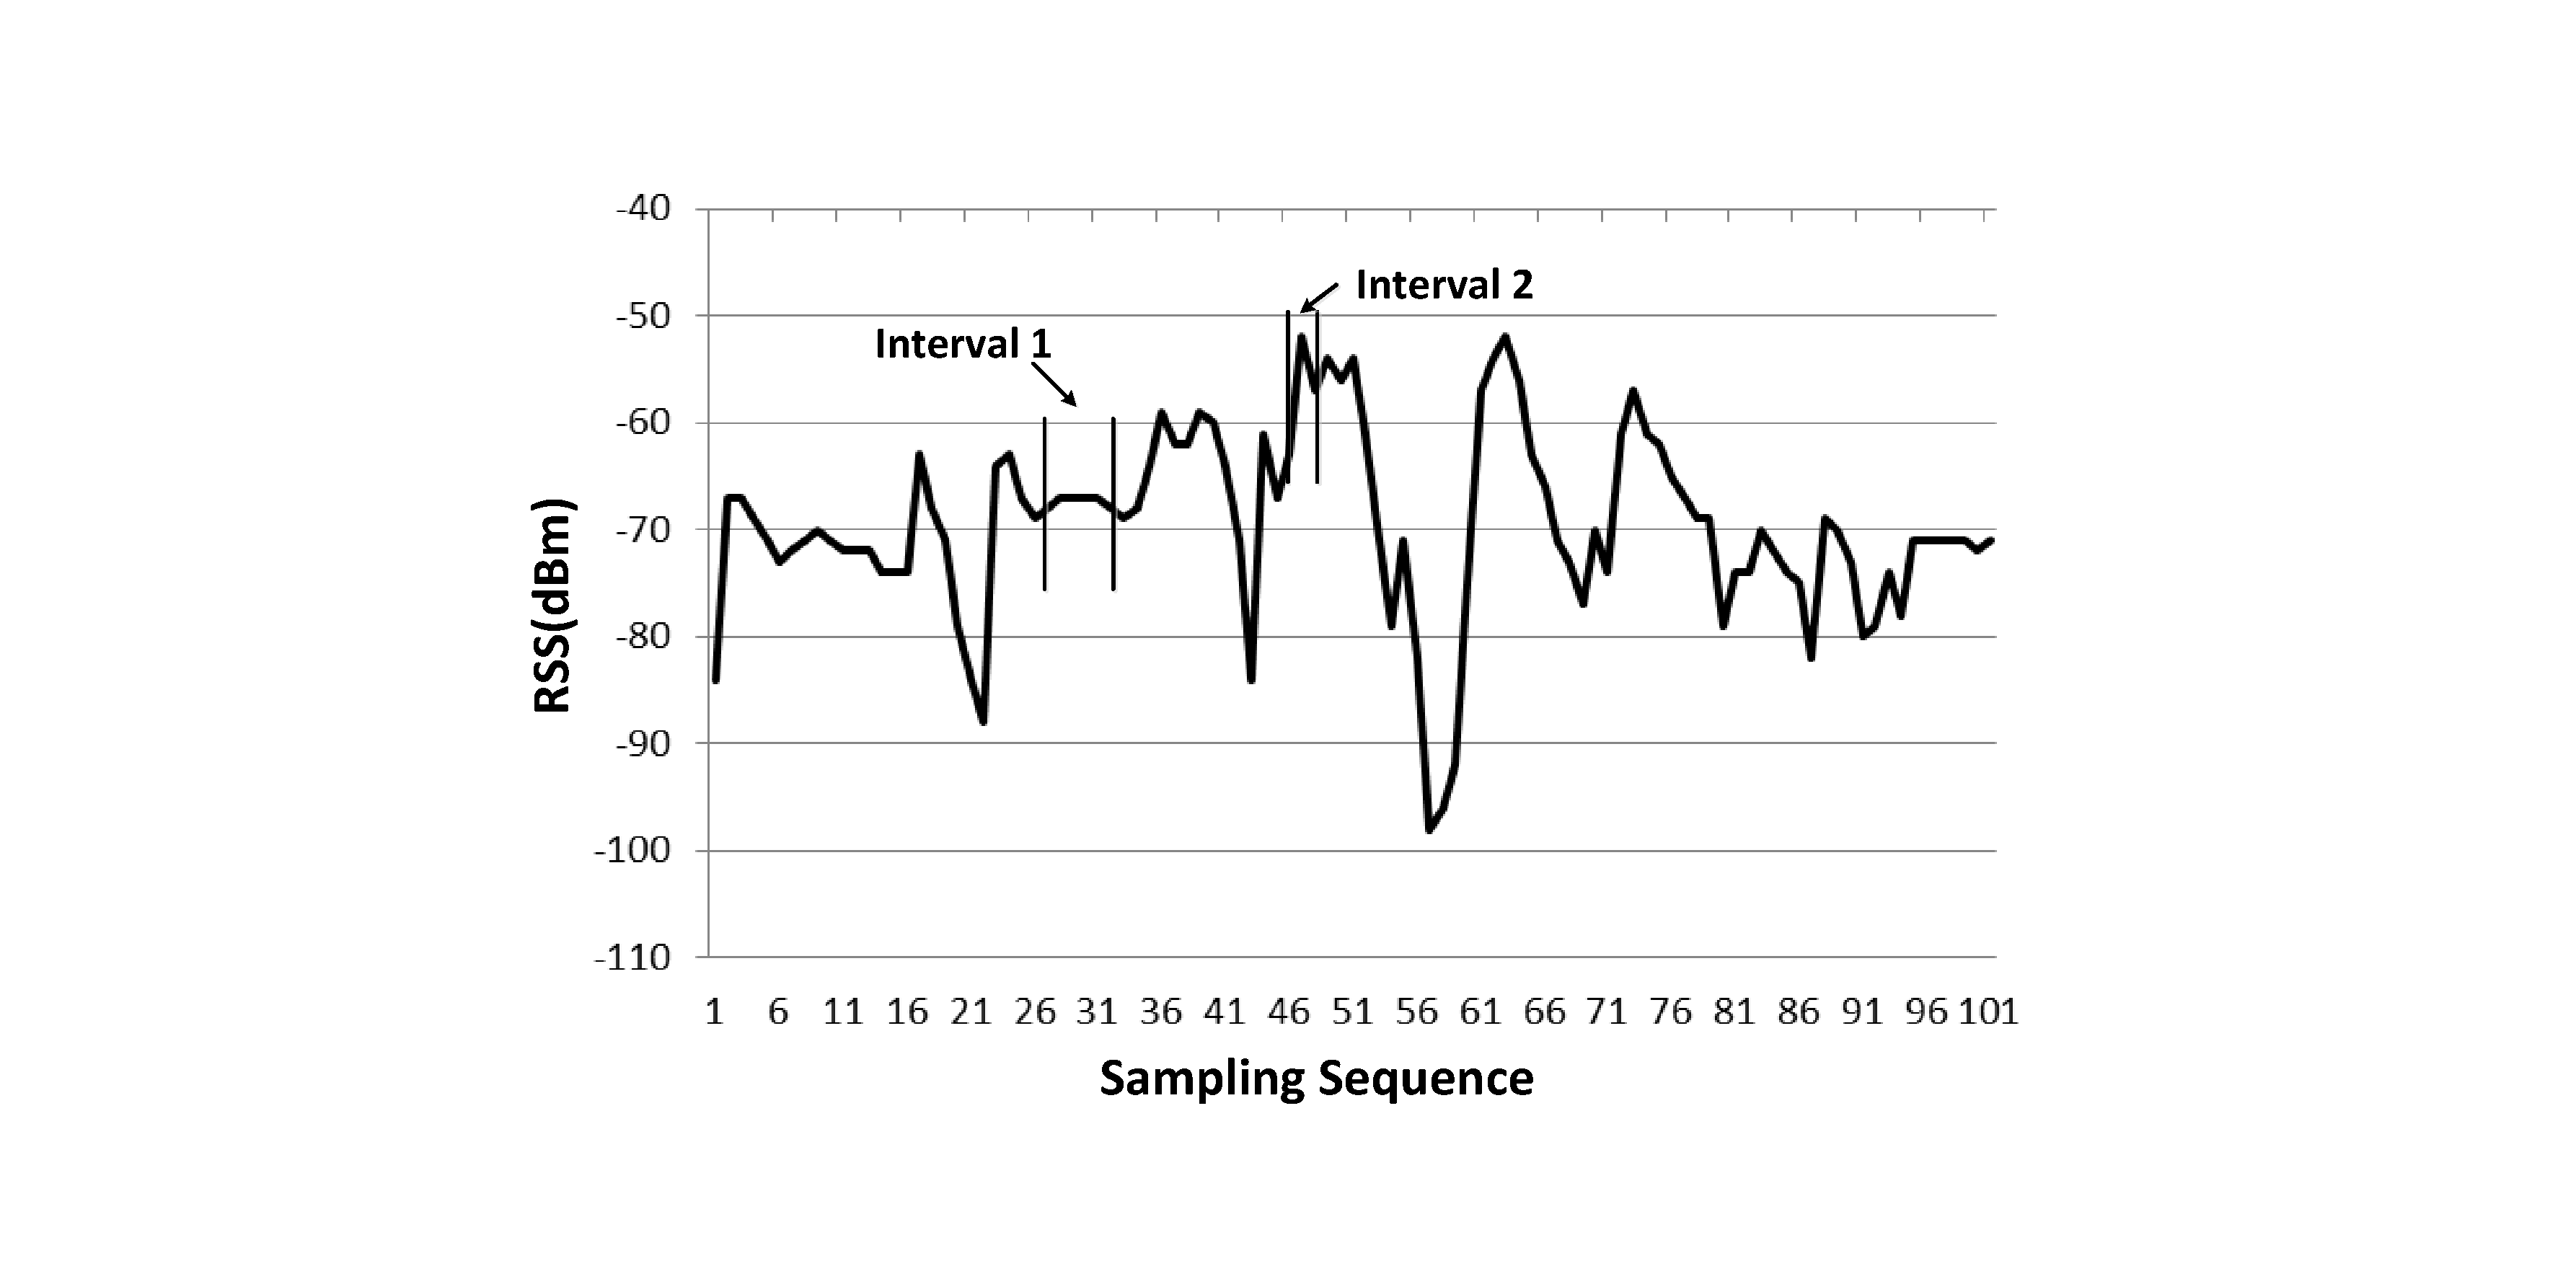
\includegraphics[width=4in]{chap2/result.pdf}
\bicaption[fig:example]{信道状态采样频率}{信道状态采样频率}{Fig}{Example of sampling frequency}
\end{figure}

The estimation results is summarized in Table~\ref{tab:summary} in detail, and it gives the length of statistical interval and number of averaging samples according to propagation environment. The type of different terrain is distinguished by Rician fading factor $K$, it is intensive areas without LOS components when $K=0$, and the propagation environment becomes more flat gradually along with the increase of $K$. The on-line estimating results are compared to Lee's method in the case of $K=0$ which means the fading channels is Rayleigh distributed, and it requires smaller sampling intervals in Lee's method. The power in the direct path increase as the terrain becomes flat, so that the number of averaging samples is less than 5 when $\nu$ becomes larger than 10, and it does not need to make frequent sampling although the length of statistical interval decreases.

%\begin{table}
%\begin{center}
%\caption{Units for Magnetic Properties}
%\label{tb:Units for Magnetic Properties}
%\begin{tabular}{lp{2.5cm}p{4.4cm}}
%\hline\hline
%\rule{-1.9mm}{3.5mm}{Symbol} & {Quantity} & {Conversion from Gaussian and CGS EMU to SI$^\texttt{a}$} \\
%\hline
%\rule{-1.9mm}{3mm}{$\Phi$} & {magnetic flux} & {1 Mx $\rightarrow$ 10$^{-8}$ Wb = 10$^{-8}$ V$\cdot$s} \\
%\rule{-1.9mm}{3mm}{\textit{B}} & {magnetic flux density, magnetic induction} & {1 G $\rightarrow$ 10$^{-4}$ T = 10$^{-4}$ Wb/m$^{2}$} \\
%\rule{-1.9mm}{3mm}{\textit{H}} & \parbox[t]{2.5cm}{\raggedright magnetic field strength} & {1 Oe $\rightarrow$ 10$^{3}$/(4$\pi$) A/m} \\
%\hline
%\hline
%\end{tabular}
%\end{center}
%No vertical lines in table. Statements that serve as captions for the entire table do not need footnote letters.
%
%$^{\texttt{a}}$Gaussian units are the same as cgs emu for magnetostatics; Mx = maxwell, G = gauss, Oe = oersted; Wb = weber, V = volt, s = second, T = tesla, m = meter, A = ampere, J = joule, kg = kilogram, H = henry.
%\end{table}

\begin{table}[!htp]
\renewcommand{\arraystretch}{1}
\bicaption[tab:summary]{信道状态估计结果总结}{信道状态估计结果总结}{Table}{Summary of Experiment Results of Channel State Estimation}
\centering
\begin{threeparttable}[b]
\begin{tabular}{c|c|c|c|c|c|c|c|c|c|c}
%\toprule
\hline
%\cline{1-11}
\multicolumn{1}{c|}{\multirow{3}{*}{Terrain}} & \multicolumn{1}{c|}{\multirow{3}{*}{$K$(dB)}} & \multicolumn{1}{c|}{\multirow{3}{*}{$\nu$}} & \multicolumn{1}{c|}{\multirow{3}{*}{$\sigma$}} & \multicolumn{1}{c|}{\multirow{3}{*}{$2L/\lambda$}} & \multicolumn{1}{c|}{\multirow{3}{*}{$N$}} & \multicolumn{1}{c|}{\multirow{3}{*}{$\Delta d/\lambda$}} & \multicolumn{1}{c|}{\multirow{3}{*}{$\Delta d$(m)}} & \multicolumn{3}{c}{$v_{train}$(km/h)}\\
\cline{9-11}
\multicolumn{1}{c|}{} & \multicolumn{1}{c|}{} & \multicolumn{1}{c|}{} & \multicolumn{1}{c|}{} & \multicolumn{1}{c|}{} & \multicolumn{1}{c|}{} & \multicolumn{1}{c|}{} & \multicolumn{1}{c|}{} & 200 & 250 & 300\\
\cline{9-11}
\multicolumn{1}{c|}{}& \multicolumn{1}{c|}{} & \multicolumn{1}{c|}{} & \multicolumn{1}{c|}{} & \multicolumn{1}{c|}{} & \multicolumn{1}{c|}{} & \multicolumn{1}{c|}{} & \multicolumn{1}{c|}{} & \multicolumn{3}{c}{$\Delta t$(ms)}\\
%\midrule[5pt]
%\hline
%\hline
\cline{1-11}
NLOS\tnote{*}  &  0 &    - & - & 40 & 36 &  1.1 & 0.367 &  2.20 &  1.76 &  1.47\\
\hline
Dense &  0 &   0 & 1 & 55 & 15 &  3.7 & 1.222 &  7.33 &  5.86 &  4.89\\
      &  2 &   4 & 2 & 18 & 12 &  1.5 & 0.500 &  3.00 &  2.40 &  2.00\\
      &  4 & 5.6 & 2 &  9 &  9 &  1.0 & 0.333 &  2.00 &  1.60 &  1.33\\
      &  6 &   6 & 3 & 20 &  7 &  2.9 & 0.967 &  5.80 &  4.64 &  3.87\\
      &  8 &  12 & 3 &  8 &  1 &  8.0 & 2.667 & 16.00 & 12.80 & 10.67\\
Open  & 10 &  18 & 4 & 12 &  1 & 12.0 & 4.000 & 24.00 & 19.20 & 16.00\\
%\bottomrule[10pt]
\hline
%\cline{1-11}
\end{tabular}
\begin{tablenotes}
\item[*] \small Caculated by Lee's method of local mean power estimation in the case of Rayleigh fading
\end{tablenotes}
\end{threeparttable}
\end{table}

\begin{figure}[!htp]
\centering
    \subfigure[接收信号强度与大尺度衰落]{
    \label{fig:input}
    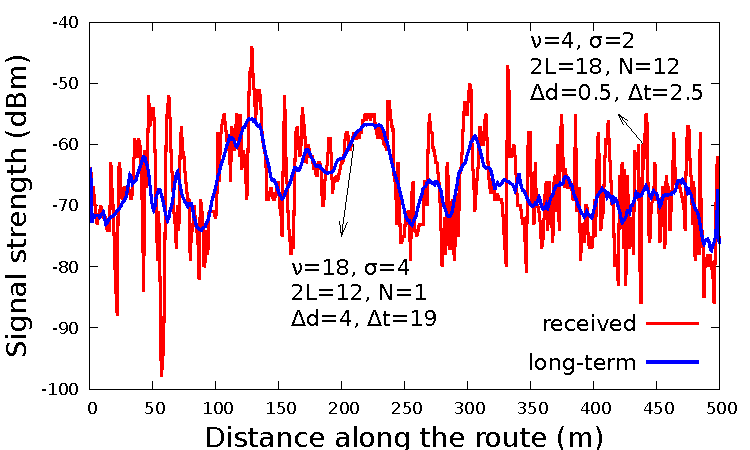
\includegraphics[width=4.5in]{chap2/em.pdf}}
\hspace{1in}
\centering
    \subfigure[小尺度衰落]{
    \label{fig:output}
    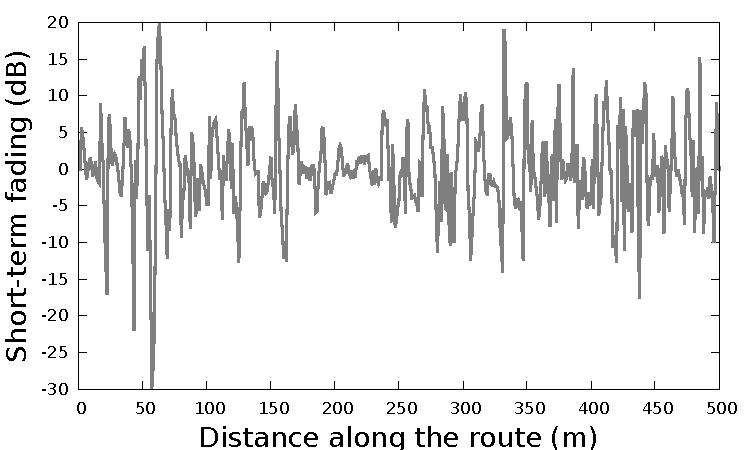
\includegraphics[width=4.5in]{chap2/short.pdf}}
\bicaption[fig:strength]{接收信号强度与信号衰落}{接收信号强度与信号衰落}{Fig}{Received signal strength and signal fading}
\end{figure}

\nocite{*}
